\documentclass{pjatk}

\usepackage{tocloft}
\usepackage{hyperref}
\usepackage[english,polish]{babel}
\usepackage{tikz-uml}
\usepackage[acronym, toc, numberedsection]{glossaries}
\usepackage{indentfirst} % wcięcie w pierwszym akapicie rozdziału
\usepackage{parskip} % przerwa między akapitami
\usepackage[defaultlines=4,all]{nowidow}
\usepackage[T1]{fontenc} % better font encoding
\usepackage{lmodern}

\glstoctrue
\clubpenalty=9996
\widowpenalty=9999
\brokenpenalty=4991
\predisplaypenalty=10000
\postdisplaypenalty=1549
\displaywidowpenalty=1602
\tolerance=1
\emergencystretch=\maxdimen
\hyphenpenalty=10000
\hbadness=10000

\addbibresource{bibliography.bip}

\makeglossaries
%! Author = Mateusz Budzisz
%! Date = 08/11/2023

\newglossaryentry{pwa}{name={Progressive Web App},
description={Progressive Web App (PWA) to progresywna aplikacja internetowa uruchamiana tak jak zwykła strona internetowa,
 ale umożliwiająca stworzenie wrażenia działania jak natywna aplikacja mobilna lub aplikacja desktopowa. }
}
\newglossaryentry{aws}{name={Amazon Web Services},
description={Amazon Web Services (AWS) – pakiet usług chmurowych oferowanych przez Amazon},
}
\newglossaryentry{gcp}{name={Google Cloud Platform},
description={Oferowany przez Google zestaw usług chmurowych, obejmuje szereg modułowych usług chmurowych, w tym przetwarzanie danych, przechowywanie danych, analitykę danych oraz uczenie maszynowe, a także zestaw narzędzi zarządzania.}
}
\newglossaryentry{azure}{ name={Azure},
description={Microsoft Azure to platforma chmurowa firmy Microsoft stworzona w modelu PaaS (Platform as a Service)}
}
\newglossaryentry{osm}{name={Open Street Map},
description={OpenStreetMap (OSM) – projekt społeczności internetowej mający na celu stworzenie darmowej, swobodnie dostępnej mapy całej kuli ziemskiej.}}
\newglossaryentry{lsp}{name={Language Service Protocol},
description={Protokół Language Server Protocol (LSP) to otwarty protokół oparty na JSON-RPC, stosowany pomiędzy edytorami kodu źródłowego lub zintegrowanymi środowiskami programistycznymi (IDE) a serwerami, które dostarczają "narzędzia inteligencji językowej": specyficzne dla języków programowania funkcje, takie jak uzupełnianie kodu, podświetlanie składni oraz oznaczanie ostrzeżeń i błędów, a także rutyny refaktoryzacji.}
}
\newglossaryentry{osw}{
name={Open Weather Map},
description={Open Weather Ma} 
}
\newglossaryentry{http}{name={Hyper Text Transfer Protocol},
description={ Hyper Text Transfer Protocol protokół stworzony przez Tima Bernersa-Lee na potrzeby komunikacji między klientem a serwerem w sieci WWW (ang. World Wide Web).}
}

\newglossaryentry{drag-n-drop}
{
    name={Drag and drop},
    description={Technologia umożliwiająca interfejsom użytkownika w przeglądarkach internetowych korzystanie z funkcji przeciągania i upuszczania elementów. Użytkownik może wybrać elementy do przeciągania za pomocą myszy, przeciągnąć te elementy do elementu docelowego i upuścić je, zwalniając przycisk myszy. Podczas operacji przeciągania półprzezroczysta reprezentacja przeciąganych elementów podąża za wskaźnikiem myszy.}
}

\newglossaryentry{on-demand}
{
    name={On-demand},
    description={Rodzaj oprogramowania charakteryzującego się dynamicznym czasem pracy, uruchamiane na rządanie, gdy poda wynik program kończy pracę zamiast oczekiwać następnego zapytania}
}

\newglossaryentry{refactoring}
{
    name={Refactoring},
    description={Znaczna zmiana konstrukcji programu mająca na celu usprawnienie oprogramowania bądź dostosowanie go do nowych wymogów}
}

\newglossaryentry{ui}
{
    name={UI},
    description={Interfejs użytkownika}
}

\newglossaryentry{frontend}
{
    name={Frontend},
    description={Oprogramowanie składające się z UI z którym docelowy użytkownik będzę wchodził w interakcję}
}

\newglossaryentry{backend}
{
    name={Backend},
    description={Oprogramowanie pozbawione UI z którym docelowy użytkownik będzę wchodził w interakcję, potrzebne do prawidłowej pracy Frontendu}
}

\newglossaryentry{job}
{
    name={Job},
    description={Oprogramowanie, które ma z góry określony cel, po jego uruchomieniu natychmiast zaczyna je wykonywać, nie wchodzi w interakcje z użytkownikiem docelowym, po zakończeniu kończy swoje życie}
}


\newglossaryentry{rendering}
{
    name={Wyrenderowanie},
    description={Stworzenie UI z postaci kodu do postaci konsumowalnej przez użytkownika docelowego}
}

\newglossaryentry{hello-world}
{
    name={Hello world},
    description={Minimalny reprezentatywny program w danej technologii}
}

\newglossaryentry{hermetyzacja}
{
    name={Hermetyzacja},
    description={Hermetyzacja opgorgramowania określa dobrą praktykę programistyczną polegającą na izolacji komponentów w aplikacji tak aby o sobie nie wiedziały gdy nie muszą o sobie wiedzieć}
}

\newglossaryentry{infra-as-code}
{
    name={Infrastructure as a code},
    description={Sposób opisania architektury systemu poprzez napisanie programu tworzącego docelową architekturę przy pomocy abstrakcji dostarczonych przez dostawcę mocy obliczeniowej}
}

\newglossaryentry{on-prem}
{
    name={On-premise},
    description={Oprogramowanie hostowane na samodzielnie zarządzanej infrastrukturze}
}

\newglossaryentry{virt}
{
    name={Wirtualizacja},
    description={Podział serwera na maszyny o mniejszej mocy obliczeniowej, aby umożliwić podział podzespołów pomiędzy klientów tak, aby nic o sobie nawzajem nie wiedzieli}
}

\newglossaryentry{arm}
{
    name={Architektura ARM},
    description={Architektura silnej ręki lol}
}
\newglossaryentry{poidef}
{
    name={POI},
    description={Point of interest (w skrócie POI) to punkt w przestrzeni, najczęściej na powierzchni Ziemi.}
}
\newglossaryentry{openlayers}
{
    name={Openlayers},
    description={OpenLayers to biblioteka napisana w języku JavaScript, ułatwiająca dodawanie dynamicznych map na stronach internetowych.}
}
\newglossaryentry{reflink}
{
    name={Reflink},
    description={Reflink to specjalny link, który zawiera unikalny kod identyfikacyjny, pozwalający na monitorowanie ruchu i przekierowań z innych źródeł.}
}
\newglossaryentry{sla}
{
    name={SLA},
    description={Service Level Agreement, SLA (umowa o gwarantowanym poziomie świadczenia usług) to umowa utrzymania i systematycznego poprawiania ustalonego między usługodawcą a usługobiorcą poziomu jakości usług poprzez stały cykl obejmując: uzgodnienia,
    monitorowanie usługi, raportowanie, przegląd osiąganych wyników.}
}
\newglossaryentry{sws}
{
    name={SWS},
    description={Specyfikacja Wymagań Systemowych }
}
\newglossaryentry{moscow}
{
    name={MoSCoW},
    description={Metoda MoSCoW to technika priorytetyzacji wykorzystywana w analizie biznesowej i przy tworzeniu oprogramowania w celu osiągnięcia wspólnego zrozumienia pomiędzy interesariuszami co do znaczenia, jakie ma dla nich dostarczenie każdego z wymagań. Inne nazwy metody to priorytetyzacja MoSCoW lub analiza MoSCoW.}
}
\newglossaryentry{CRUD}
{
    name={CRUD},
    description={CRUD (od angielskiego create, read, update, delete, tłumaczenie utwórz, odczytaj, aktualizuj, usuń) – cztery podstawowe funkcje w aplikacjach korzystających z bazy danych, które umożliwiają zarządzanie nią.}
}
\newglossaryentry{stadiamaps}
{
    name={Stadia Maps},
    description={Stadia Maps oferuje komercyjne interfejsy API do mapowania i wyznaczania tras, głównie oparte na OpenStreetMap.}
}

\newglossaryentry{mevo}
{
    name={Mevo},
    description={Mevo to system bezobsługowych wypożyczalni rowerów miejskich.}
}
\newglossaryentry{scraping}
{
    name={Web scraping},
    description={Data scraping to technika ekstrakcji danych z witryn internetowych.}
}
\newglossaryentry{lighthouse}
{
    name={Lighthouse},
description={Lighthouse to narzędzie open-source stworzone przez Google do automatycznego audytu stron internetowych. Analizuje wydajność, dostępność, zgodność z progresywnymi aplikacjami webowymi (PWA), SEO i najlepszymi praktykami. Wyniki audytów pomagają poprawić jakość i funkcjonalność stron internetowych. Narzędzie można uruchomić z poziomu Chrome DevTools, jako rozszerzenie Chrome lub z wiersza poleceń.}
}
\newglossaryentry{openmeteo}
{
    name={OpenMeteo},
description={OpenMeteo to darmowa, otwarta usługa dostarczająca prognozy pogody poprzez interfejs API. Oferuje precyzyjne prognozy dla różnych lokalizacji na świecie, umożliwiając integrację z aplikacjami i serwisami internetowymi.}
}


\studfield{Informatyka}
\studtype{Zaoczne}
\title{Planer Mapy Miejskiej}
\engtitle{City Map Planner}
\acronym{City Planner}
\titledate{2023-10-14}
\supervisor{prof. dr hab. Marek A. Bednarczyk}
\author{Mateusz Budzisz}{s24048}{Aplikacje Internetowe}{Zaoczny}
\author{Wiktor Rostkowski}{s23141}{Aplikacje Internetowe}{Zaoczny}
\author{Sebastian Kreft}{s23133}{Aplikacje Internetowe}{Zaoczny}
\author{Damian Kreft}{s23447}{Aplikacje Internetowe}{Zaoczny}
\consultant{--- brak ---} % Koniecznie trzeba podać brak, albo wpisać konsultantów tak jak przy autorach
\projectgoals{Stworzenie interaktywnej mapy miejskiej do planowania zwiedzania atrakcji turstycznych z wkykorzystaniem dynamicznych danych}
\productsandservices{Aplikacja progresywana}
\mainfunctionalities{Planowanie trasy}
\successmeasure{Wdrożenie rozwiązania jako oficjalnego rozwiązania miejskiego}
\projlimitations{Brak budżetu}
\date{\today}
\nabstract{
	Praca zakłada utworzenie interaktywnej mapy z punktami zainteresowań na podstawie listy atrakcji turystycznych wyróżnionych przez urząd miejski,
	umożliwiającej kompleksowe zaplanowanie optymalnej trasy zwiedzania z uwzględnieniem środków komunikacji miejskiej,
	godzin otwarcia atrakcji turystycznych oraz warunków pogodowych.
}

\graphicspath {{attachments/}}

\begin{document}

	% PJATK Template begin
	\maketitle
	\makeprojectcard
	\makedeclaration
	% PJATK Template End

    % Spis treści
	\tableofcontents
	\clearpage

    % \include{chapters/przykłady-latex}
	%! Author = Wiktor Rostkowski, Mateusz Budzisz
%! Date = 29.10.2023

\chapter{Wstęp}
\label{ch:wstep}

W miastach, które oferują wiele atrakcji turystycznych oraz posiadają rozbudowane~i~złożone systemy transportu publicznego, tworzenie optymalnego planu zwiedzania może~być~skomplikowane~i~czasochłonne.
Konieczność uwzględnienia godzin otwarcia poszczególnych miejsc, dostępności różnych środków transportu oraz efektywnego wykorzystania czasu sprawia,~że~planowanie wycieczki wymaga dużej precyzji~i~uwagi.
Co więcej, uwzględnienie indywidualnych preferencji turystów, takich~jak~zainteresowania, tempo zwiedzania~czy~potrzeba przerw~na~odpoczynek, jeszcze bardziej zwiększa stopień trudności tego zadania.

Zespół projektowy wcześniej napotkał dokładnie~ten~problem,~co~doprowadziło~do~powstania pomysłu~na~stworzenie nowatorskiej aplikacji.
Aplikacja~ta~składa~się~z interaktywnej mapy, która prezentuje różnorodne atrakcje turystyczne~w~danym mieście, oraz kalendarza~w~stylu \gls{drag-n-drop}, umożliwiającego łatwe planowanie dnia.
Aplikacja uwzględnia dane~w~czasie rzeczywistym, takie~jak~prognoza pogody, aktualne informacje~o~komunikacji miejskiej oraz godziny otwarcia poszczególnych atrakcji.
Ponadto aplikacja oferuje interaktywny widok, który automatycznie generuje optymalną trasę zwiedzania zgodnie~z~ustalonym planem, wspierając użytkowników~w~maksymalnym wykorzystaniu~ich~czasu~i~zasobów podczas wizyty~w~mieście.

Niniejszy dokument przedstawia szczegółowy proces powstawania opisanego rozwiązania, rozpoczynając~od~przedstawienia~i~omówienia problemu, kontekstu oraz zakresu systemu,~a~także omówienia wymagań.
Następnie przedstawione~są~kluczowe decyzje projektowe, które kształtowały architekturę systemu, oraz szczegółowy opis procesu implementacji, obejmujący realizację poszczególnych modułów.
W kolejnej części pracy omawiany jest proces testowania,~w~tym metody~i~narzędzia używane~do~zapewnienia jakości~i~niezawodności systemu.
Zakończenie pracy obejmuje prezentację osiągniętych rezultatów oraz~ich~analizę,~a~także podsumowanie całości projektu.
Warto zaznaczyć,~że~praca początkowo była realizowana przez czteroosobowy zespół, jednak~pod~sam koniec projektu dwie osoby zdecydowały~się~zrezygnować~z~dalszego udziału,~co~wpłynęło~na~ostateczny przebieg~i~realizację projektu.

	%! Author = Wiktor Rostkowski, Mateusz Budzisz
%! Date = 05/1/2024

\chapter{Opis problemu}
\label{ch:opis-problemu}

\section{Przestawienie problemu}
\label{sec:przestawienie-problemu}

Analizując swoje potrzeby jako turystów, zespół projektowy zauważył liczne obszary,~w~których aplikacja może znacząco wspierać turystów.
W trakcie~tej~analizy, członkowie zespołu zidentyfikowali konkretne wyzwania~i~problemy,~z~jakimi turyści często~się~borykają.

Pierwszą kwestią jest natłok informacji, który może przytłoczyć turystów.
Podczas poszukiwania informacji~o~atrakcjach turystycznych, turyści~są~bombardowani ogromną ilością niepotrzebnych danych, takich~jak~punkty zainteresowań, które~w~rzeczywistości~nie~są atrakcjami turystycznymi.
Na przykład, korzystając~z~map Google, Bing~lub~Apple, użytkownicy często otrzymują wyniki, które oprócz rzeczywistych atrakcji turystycznych, zawierają również miejsca niezwiązane~z~turystyką, takie~jak~stacje benzynowe, szpitale~i~inne obiekty użyteczności publicznej.
Taka sytuacja utrudnia szybkie~i~efektywne znalezienie informacji~o~faktycznych atrakcjach, powodując frustrację~i~dezorientację użytkowników.
Dlatego niezwykle ważne jest,~aby~aplikacja skierowana~do~turystów była~w~stanie filtrować~i~precyzyjnie dostarczać informacje, które~są~istotne~i~wartościowe~z~punktu widzenia osób podróżujących.

Kolejnym problematycznym obszarem jest dostęp~do~godzin otwarcia~i~aktualność tych danych, które często~są~powielone~w~różnych wersjach~w~wielu miejscach.
Turystom zdarza~się~spotkać~z~rozbieżnościami~w~informacjach~na~temat godzin otwarcia muzeów, parków, restauracji~i~innych atrakcji turystycznych.
Na przykład, godziny otwarcia podane~na~oficjalnej stronie internetowej mogą różnić~się~od tych zamieszczonych~na~platformach społecznościowych, portalach recenzji~lub~w przewodnikach turystycznych.
Takie niespójności mogą prowadzić~do~nieporozumień~i~frustracji, kiedy turyści pojawiają~się~w miejscu, które miało~być~otwarte,~ale~okazuje~się~zamknięte.
Dlatego ważne jest,~aby~aplikacja~dla~turystów mogła zapewniać zaktualizowane, spójne~i~wiarygodne informacje~o~godzinach otwarcia, minimalizując ryzyko takich problemów~i~ułatwiając planowanie zwiedzania.

Trzecim~z~problematycznych obszarów jest skomplikowanie rozłożenia zwiedzania~na~poszczególne dni.
Ręczne tworzenie takiego planu wymaga zaawansowanych zdolności analitycznych oraz dużego nakładu pracy,~a~mimo~to~jest bardzo podatne~na~błędy.
Tworzony~w~ten sposób plan często szybko~się~dezaktualizuje,~co~wymusza konieczność jego ponownego przemyślenia~i~wykonania~od~nowa.
Chociaż istnieją narzędzia wspomagające planowanie dnia, konieczność ręcznego wprowadzania godzin otwarcia atrakcji turystycznych sprawia,~że~ich użycie może~być~bardziej czasochłonne~niż~przynoszące korzyści.
W efekcie, zamiast ułatwiać planowanie, narzędzia~te~często komplikują proces, zniechęcając użytkowników~do~ich stosowania.
Aby rzeczywiście wspomóc turystów~w~efektywnym planowaniu, aplikacja powinna automatycznie integrować aktualne informacje~o~godzinach otwarcia, dostarczając kompleksowe~i~łatwe~w~użyciu narzędzie~do~tworzenia planów zwiedzania.
Dzięki temu turyści będą mogli skupić~się~na cieszeniu~się~podróżą,~a~nie~na~logistyce~jej~organizacji.

Ostatnim obszarem wymagającym usprawnień jest ułożenie trasy~z~wykorzystaniem komunikacji miejskiej pomiędzy wieloma punktami.
Gdy użytkownik stworzy plan zwiedzania, powinien mieć automatyczną możliwość zobaczenia dostępnych połączeń między wybranymi atrakcjami~bez~konieczności ręcznego wyszukiwania informacji~o~dostępnych środkach transportu.
Wprowadzenie takiej funkcji~w~aplikacji turystycznej znacznie ułatwiłoby podróżowanie, eliminując potrzebę czasochłonnego~i~często skomplikowanego poszukiwania informacji~o~trasach, rozkładach jazdy~i~przesiadkach.
Automatyczna integracja danych~o~komunikacji miejskiej zapewniłaby turystom łatwy dostęp~do~aktualnych~i~precyzyjnych informacji,~co~przyczyniłoby~się~do bardziej efektywnego planowania czasu oraz zwiększenia komfortu podróżowania.
Dzięki temu turyści mogliby skupić~się~na zwiedzaniu~i~czerpaniu przyjemności~z~odkrywania nowych miejsc, mając pewność,~że~aplikacja zadba~o~logistyczne aspekty~ich~podróży.

\section{Rich picture}
\label{sec:rich-picture}

Rich picture, czyli wzbogacony wizerunek, jest graficznym przedstawieniem problemu, które ilustruje różnorodne aspekty i zależności związane z danym zagadnieniem.
Poniżej znajduje się graficzne ujęcie problemów napotykanych przez turystów~\ref{fig:rich-picture}.

\begin{figure}[h]
    \centering
    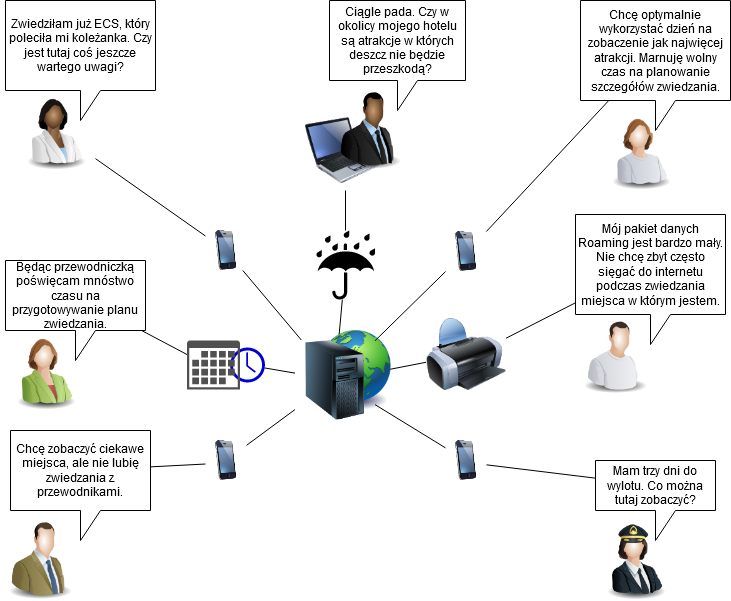
\includegraphics[width=1\textwidth]{attachments/rich-picture}
    \caption{Wzbogacony wizerunek planeru miejskiego}
    \label{fig:rich-picture}
\end{figure}

\section{Cele projektu}
\label{sec:cele-projektu}

TODO


	% Słownik pojęć i skrótów
	\printglossary[type=\acronymtype]
	\printglossary

	%! Author = Wiktor Rostkowski, Mateusz Budzisz
%! Date = 05/24/2024

\chapter{Kontekst projektu}
\label{ch:kontekst-projektu}

\section{Aspekty społeczne}
\label{sec:aspekty-spoleczne}

W erze „fake news”, gdzie występuje duża ilość niskiej jakości informacji, trudno znaleźć wiarygodne źródła informacji.
Konieczne jest wielokrotne weryfikowanie źródeł przez każdą grupę społeczną,~od~młodzieży~po~seniorów~\cite{fakenews}.

\indent Nasza aplikacja spełnia liczne potrzeby turystów pragnących efektywnie zaplanować zwiedzanie miasta wykorzystując rzetelne~i~pewne informacje~o~jego atrakcjach,~a~także~bez~znacznego nakładu czasowego.
Turystyczny planer miejski oferuje kompleksowy zbiór informacji niezbędnych~dla~każdego turysty, wolny~od~niedopowiedzeń.
Przewidywaną grupą docelową~są~osoby odwiedzające daną miejscowość, posiadające umiarkowaną znajomość technologii, które chcą dostosować podróż zarówno~dla~siebie,~jak~i~dla~większych grup,~na~przykład wycieczek~dla~znajomych.

\indent Na~potrzeby turystów proponowane jest rozwiązanie~z~następującymi funkcjami:

\begin{enumerate}
    \item Interaktywna mapa~z~naniesionymi atrakcjami turystycznymi zawierająca zawsze aktualne informacje~o~atrakcjach turystycznych.
    \item Generowanie planu wycieczki~na~podstawie wybranych miejsc oraz trasy pomiędzy nimi.
    \item Automatyczna aktualizacja planu zwiedzania~na~podstawie dynamicznych wydarzeń, takich~jak~zmiana pogody, rozkład jazdy~czy~dostępność atrakcji,~co~umożliwia planowanie~w~czasie rzeczywistym.
\end{enumerate}

Dzięki~tym~funkcjonalnościom możliwe jest uniknięcie wielogodzinnego poszukiwania informacji~na~temat dostępnych miejsc oraz efektywne zaplanowanie podróży.

\indent Przeanalizowano społeczne aspekty wdrożenia proponowanego rozwiązania,~w~wyniku czego zidentyfikowano zarówno pozytywne,~jak~i negatywne skutki.

\indent Jednym~z~założeń projektu jest wspieranie rozwoju turystyki.
Aplikacja promuje niszowe atrakcje, prezentując~na~mapie tylko wybrane miejsca.
Dzięki mniejszej liczbie znaczników, mniej popularne atrakcje mają większą szansę~na~znalezienie przez użytkowników.

\indent Przedstawione informacje~są~dostępne~dla~każdego odwiedzającego~i~obejmują~nie~tylko atrakcje turystyczne,~ale~także dostępny transport,~a~w przyszłości również zakwaterowanie~i~restauracje.
Dzięki temu podróżowanie staje~się~łatwiejsze~i~nie wymaga posiadania przewodnika,~a~samodzielna koordynacja~nie~wiąże~się~z nadmiernym obciążeniem poznawczym. \newline
Człowiek podczas zwiedzania miasta skupia~się~na doświadczaniu~i~zwiedzaniu,~a~nie selekcjonowaniu danych, informacji~i~podejmowaniu decyzji.
Aplikacja zapobiega obciążeniu poznawczemu (ang.\ cognitive load), które jest konsekwencją nadmiaru opcji dostępnych~w~danym mieście.
Dzięki "uwolnionym zasobom" możliwa jest koncentracja użytkowników~na~faktycznym poznawaniu miasta~\cite{cognitive-biases}.

\indent Dodatkowo, rezygnacja~z~przetwarzania danych wrażliwych~w~przyjętym modelu zwiększa poczucie bezpieczeństwa użytkowników.
Korzystanie~z~systemu~nie~wiąże~się~z ryzykiem utraty~lub~nieuprawnionego wykorzystania danych,~co~jest kluczowe~dla~zachowania zaufania.
Celem jaki towarzyszył zespołowi projektowemu, było zaspokajanie potrzeb użytkowników, uwzględniając~ich~interesy oraz przestrzeganie obowiązującego prawa, przy jednoczesnym zachowaniu poufności.

\indent Wytworzona aplikacja pozwala użytkownikom łatwo~i~samodzielnie uzyskać dostęp~do~trudno dostępnych informacji.
Dzięki wygodnemu planowaniu~w~formie interfejsu drag-and-drop, aplikacja zmniejsza atrakcyjność płatnych przewodników oferujących gotowe plany zwiedzania
W rezultacie może~to~generować negatywne konsekwencje społeczne~w~postaci zwiększonego poczucia zagrożenia wśród przewodników turystycznych działających~na~wolnym rynku.

\indent Warto również wspomnieć,~że~podczas implementacji aplikacji,~z~powodu braku czasu, pominięto kilka funkcji, które~w~aktualnej wersji mogą generować potencjalne niezadowolenie użytkowników.
Na przykład, brak możliwości rezerwacji terminów~w~wybranych atrakcjach może~być~problematyczny~dla~użytkowników, szczególnie~gdy~wymagana jest wcześniejsza rezerwacja.
Ponadto,~nie~zdążono dodać integracji~z~zakwaterowaniem~i~lokalami gastronomicznymi.
Niemniej jednak, aplikacja została przystosowana~dla~osób~z~wadami wzroku,~co~stanowi istotny krok~w~kierunku zwiększenia~jej~dostępności~i~inkluzywności.

\indent W~związku~z~powyższym zidentyfikowano obszary wymagające udoskonalenia proponowanego systemu,~aby~skuteczniej odpowiadał~na~potrzeby użytkowników oraz wywierał większy wpływ społeczny.
Kluczowym aspektem~z~perspektywy społecznej~w~przyszłości będą elementy sieci społecznościowej, takie~jak~recenzje atrakcji turystycznych oraz możliwość dzielenia~się~planami zwiedzania~z~innymi użytkownikami.



\pagebreak
\section{Analiza ryzyka}
\label{sec:analiza-ryzyka}

\begin{longtable}{|p{.1\linewidth}|p{.15\textwidth}|p{.2\textwidth}|p{.25\textwidth}|p{.25\textwidth}|}
    \hline
    Ryzyko & Czynniki ryzyka & Charakterystyka ryzyka & Prawdopodobieństwo wystąpienia ryzyka & Planowane działania \\
    \hline
    \multirow{6}{=}{\parbox[c]{12cm}{\rotatebox[origin=c]{90}{\multirow{6}{=}{\textbf{Nieukończenie projektu w terminie}}}}}& Rozpad grupy & Odejście jednego z członków zespołu & niskie
    & Przejrzysta komunikacja w zespole i ustalenie wersji MVP produktu, która może zostać ukończona w uszczuplonym składzie \\
    \cline{2-5}
    & Czasowa niedostępność / niedyspozycja członka zespołu & Nagła lub zaplanowana nieobecność członka zespołu & średnie
    & Możliwie wczesne sygnalizowanie planowanej nieobecności \\
    \cline{2-5}
    & Zbyt ambitne założenia projektowe & Zaplanowane prace wykraczają poza moce przerobowe członków zespołu & średnie
    & Śledzenie postępu prac pod kątem wykonalności i zmieszczenia się w ograniczeniach czasowych, konsultacja z promotorem \\
    \cline{2-5}
    & Pełzające wymagania & Ciągle powiększana pula wymagań, zwiększająca zakres prac do wykonania & średnie & Iteracyjna implementacja i dopracowywanie wymagań pod implementację \\
    \cline{2-5}
    & Nauka nowych technologii / języków programowania & Zwiększenie ilości czasu potrzebnej na ukończenie zadania &
    wysokie & Używanie technologii opanowanych przez zespół projektowy \\
    \cline{2-5}
    & Problem z komunikacją w zespole & Brak właściwego przepływu informacji między członkami zespołu & średnie
    & Cykliczne spotkania członków zespołu w celu omawiania postępu prac i planowania kolejnych działań \\
    \hline
    \pagebreak
    \hline
    \multirow{5}{=}{\parbox[c]{10cm}{\rotatebox[origin=c]{90}{\multirow{5}{=}{\textbf{Produkt nie spełnia wymagań projektowych}}}}} & Błędna analiza rynku & Niewłaściwe rozpoznanie potrzeb potencjalnych użytkowników oraz rozwiązań konkurencyjnych & niskie
    & Konsultacje z promotorem, stworzenie profilu docelowego użytkownika \\
    \cline{2-5}
    & Niespełnienie wymagań klientów & Finalny produkt nie zapewnia zakładanych korzyści dla użytkownika końcowego & średnie
    & Konsultacje z promotorem, cykliczna analiza kierunku rozwoju produktu \\
    \cline{2-5}
    & Wydanie wersji zawierającej krytyczne błędy & Produkt zawiera błędy uniemożliwiające korzystanie z jego podstawowych funkcjonalności & niskie
    & Napisanie odpowiednich testów sprawdzających działanie funkcjonalności \\
    \cline{2-5}
    & Zmiany w usługach zależnych & Wyłączenie lub zmiana warunków na jakich udostępniane są API wpływa na dostarczane funkcjonalności & średnie
    & Ustalenie alternatywnych dostawców potrzebnych usług \\
    \cline{2-5}
    & Zły dobór narzędzi projektowych & Wybrane narzędzia są nieodpowiednie do zaplanowanych prac & niskie
    & Zaznajomienie się z dokumentacją używanych narzędzi, konsultacje w zespole \\
    \hline
    \pagebreak
    \hline
    \multirow{2}{=}{\parbox[c]{3.5cm}{\rotatebox[origin=c]{90}{\multirow{2}{=}{\textbf{Niewłaściwe zaplanowanie przebiegu prac}}}}} & Przyjęcie nieodpowiedniej strategii projektowej & Przyjęta strategia nie pozwala na uzyskanie wymaganych rezultatów przy dostępnych zasobach & wysokie
    & Stałe monitorowanie kierunku prac, konsultacje z promotorem \\
    \cline{2-5}
    & Nierozpatrzenie potencjalnych przypadków brzegowych & Konieczność uwzględnienia nieprzewidzianych prac & wysokie
    & Staranne analizowanie planowanych funkcjonalności i ich wpływu na produkt \\
    \hline
    \multirow{1}{=}{\parbox[c]{3.5cm}{\rotatebox[origin=c]{90}{\multirow{1}{=}{\textbf{Zdarzenia nieprzewidziane}}}}}& Zbyt gwałtowny rozrost liczby użytkowników & Liczba użytkowników przekracza zaplanowane możliwości techniczne produktu & niskie
    & Projektowanie produktu z możliwością jego skalowania \\
    \hline

\end{longtable}
\pagebreak
\section{Rozwiązania konkurencyjne}
\label{sec:rozwiazania-konkurencyjne}
Na rynku dostępne~są~obecnie różne rozwiązania mające~na~celu ułatwienie planowania podróży~i~posiadające różny zakres funkcjonalności.
Użytkownik może napotkać rozbudowane aplikacje integrujące wiele funkcjonalności takich~jak~układanie list atrakcji~do~zwiedzania, optymalizacja tras podróży, dokumentowanie poniesionych wydatków, tworzenie list ułatwiających planowanie (listy czynności~do~wykonania, listy zakupów, listy ułatwiające organizację pakowania), synchronizacja naszych planów podróży~ze~znajomymi, integrowanie rezerwacji hotelowych~i~lotów.
Aplikacje skupiające~się~na wspomaganiu procesu zwiedzania sugerują użytkownikowi interesujące punkty~w~jego lokalizacji (interesujące miejsca, hotele, restauracje, sklepy itp.)~i~oznaczają~je~na mapie.
Dodatkowo bardzo często~są~wyposażone~w~rozbudowany opis danej atrakcji, czasem również~w~formie głosowej,~co~umożliwia zamienienie urządzenia mobilnego~w~osobisty audio przewodnik.
Kolejną funkcjonalność stanowi możliwość dokonywania zakupu biletów~i~rezerwowania atrakcji bezpośrednio~z~poziomu aplikacji turystycznej.
Poniżej przedstawiono przykłady najpopularniejszych obecnie rozwiązań ułatwiających planowanie zwiedzania.

\subsection{Wanderlog}
\label{subsec:wanderlog}
Jest~to~aplikacja reklamująca~się~jako planer podróży,~ze~szczególnym naciskiem~na~organizowanie wakacji oraz wycieczek samochodem.
W wersji podstawowej jest darmowa, posiada również płatną wersję premium  oferującą dodatkowe funkcjonalności.
Aplikacja jest dostępna poprzez przeglądarkę internetową~jak~również poprzez dedykowaną aplikację~na~urządzenia mobilne.
Wanderlog umożliwia układanie list~z~interesującymi użytkownika miejscami~i~wydarzeniami, które~są~graficznie przedstawione~w~postaci pinezek~na~mapie google.
Po wybraniu lokalizacji~i~daty podróży, użytkownik może dokonać przeglądu ofert noclegów.
Aplikacja umożliwia tworzenie planów podróży razem~z~innymi użytkownikami oraz~ich~synchronizację~w~czasie rzeczywistym.
Ponadto użytkownik~ma~dostęp~do~spersonalizowanych sugestii.

\subsection{TripIt}
\label{subsec:tripit}
Jest~to~planer podróży integrujący wiele funkcjonalności~w~celu maksymalnego ułatwienia użytkownikowi procesu podróżowania.
Stanowi alternatywę~dla~wspomnianej wcześniej aplikacji Wanderlog~i~również posiada darmową wersję podstawową oraz wersję płatną opartą~na~modelu subskrypcyjnym, która posiada dodatkowe funkcjonalności.
W wersji podstawowej użytkownik~ma~możliwość układania planów podróży, które~są~dostępne~na~wielu urządzeniach jednocześnie.
Udostępnia statystyki, wytyczne dotyczące restrykcji COVID-19 oraz umożliwia dodawanie zdjęć, kodów~QR~oraz plików~PDF~do planów podróży.
Aplikacja zapewnia nawigację między punktami, mapy lotnisk, sugestie~co~do interesujących miejsc blisko lokalizacji użytkownika,~jak~również informowania~o~poziomie niebezpieczeństwa danej okolicy.
Podstawowa wersja aplikacji umożliwia również dzielenie~się~planami~z~innymi użytkownikami oraz synchronizację kalendarza.
W wersji płatnej użytkownik~ma~dostęp~do~szeregu funkcjonalności ułatwiających podróżowanie samolotem, np.~informacja~o~dostępności lepszych miejsc, przypomnienia~o~zarezerwowanych lotach, powiadomienia~o~statusie lotów~w~czasie rzeczywistym, mapy lotnisk wraz~ze~szczegółowymi informacjami~o~położeniu obiektów, informacje~o~punkcie odbioru bagażu.

\subsection{Harmony}
\label{subsec:harmony}
Umożliwia tworzenie planów podróży wraz~ze~znajomymi~w~czasie rzeczywistym oraz synchronizację~z~kalendarzem Google.
Ponadto aplikacja umożliwia śledzenie poniesionych wydatków~i~podziału kosztów~na~poszczególne osoby.
Użytkownik~ma~możliwość otrzymywania sugestii generowanych przez~AI~dotyczących interesujących miejsc~w~danej lokalizacji,~jak~również rezerwowania wycieczek~w~aplikacji.
Aplikacja umożliwia również tworzenie list rzeczy~do~wykonania~w~celu łatwego śledzenia postępów.
Obiekty~do~zwiedzania~są~zwizualizowane~na~mapie Google~w~postaci pinezek.

\subsection{Rove.me}
\label{subsec:rove.me}
Jest~to~aplikacja, która sugeruje użytkownikowi najlepszy czas~na~odwiedzenie danego miejsca~lub~wydarzenia~w~ciągu roku.
Aplikacja informuje również~o~typowej pogodzie występującej~w~interesującym użytkownika miejscu~z~uwzględnieniem pory roku~lub~daty.

\subsection{Roadtrippers}
\label{subsec:roadtrippers}
Umożliwia tworzenie planów podróży~ze~szczególnym uwzględnieniem podróży samochodem.
Poprawione zdania z uwzględnieniem "aplikacja":

Użytkownik oznacza~na~mapie interesujące~go~miejsca, takie jak atrakcje, hotele, stacje paliw, sklepy itp.
Aplikacja udostępnia informacje~o~odległości~od~celu podróży~i~szacowanym czasie dotarcia~do~niego.
Aplikacja skierowana jest~do~użytku~na~terenie Stanów Zjednoczonych.

\subsection{Visit a City}
\label{subsec:visit-a-city}
Użytkownik~ma~możliwość tworzenia list obiektów~do~zwiedzania,~jak~również rezerwowania wycieczek~i~aktywności~w~oparciu~o~dużą bazę dostępnych lokalizacji.
Posiadają~one~rozbudowane informacje~i~oceny dodawane przez innych użytkowników,~na~podstawie których możliwe jest dokonywanie wyborów, ponadto aplikacja sugeruje interesujące miejsca~w~pobliżu lokalizacji użytkownika.
Aplikacja jest dostępna mobilnie~na~urządzeniach~z~systemem~iOS~i Android.

\subsection{SmartGuide}
\label{subsec:smartguide}
Zamysłem aplikacji jest dostarczenie użytkownikom platformy dzięki, której urządzenie osobiste może zostać zamienione~w~przewodnik turystyczny.
Zwiedzanie odbywa~się~po zaplanowanych trasach,~a~dzięki śledzeniu lokalizacji użytkownika~za~pomocą nawigacji GPS, aplikacja może określić, kiedy osoba zwiedzająca dotarła~do~interesującego punktu~i~odtworzyć zapis audio~z~opisem obiektu.
Informacje~o~oglądanym obiekcie dostępne~są~również~w~formie tekstowej.
Aplikacja skierowana jest~nie~tylko~do~turystów,~ale~również~do~organizatorów wycieczek, którzy mogą tworzyć własne trasy zwiedzania.

\subsection{Fodor's City Guide}
\label{subsec:fodor's-city-guide}
Aplikacja rekomenduje użytkownikowi najciekawsze miejsca~do~zwiedzania oraz najlepsze restauracje, hotele~i~sklepy,~jak~również umożliwia rezerwację tych usług jest dostępna jest~na~urządzeniach~z~systemem iOS\@.

\subsection{Tripadvisor}
\label{subsec:tripadvisor}
Aplikacja umożliwia planowanie wycieczek, rezerwację usług ~w~oparciu między innymi~o~rekomendacje, opinie oraz wskazówki innych użytkowników.
Rekomendowane miejsca znajdujące~się~w~pobliżu lokalizacji użytkownika~są~przedstawione~na~mapie~w~formie pinezek.
Aplikacja umożliwia również dostęp~do~zakupionych biletów~w~formie elektronicznej.
Jest dostępna~na~urządzeniach~z~systemem~iOS~i~Android.

\subsection{Podsumowanie}
\label{subsec:podsumowanie}
W tabeli poniżej przedstawiono szczegółowe porównanie wszystkich konkurencyjnych rozwiązań, uwzględniając ich główne funkcje.

\newgeometry{top=0.5cm,bottom=0.5cm,left=2.7cm,right=0.5cm}
\begin{landscape}

    \begin{longtable}{|>{\raggedright\arraybackslash}p{5cm}|>{\centering\arraybackslash}p{1.5cm}|>{\centering\arraybackslash}p{1.5cm}|>{\centering\arraybackslash}p{1.5cm}|>{\centering\arraybackslash}p{1.5cm}|>{\centering\arraybackslash}p{1.5cm}|>{\centering\arraybackslash}p{1.5cm}|>{\centering\arraybackslash}p{1.5cm}|>{\centering\arraybackslash}p{1.5cm}|>{\centering\arraybackslash}p{1.5cm}|}
        \hline
        \textbf{Funkcjonalności} & \textbf{Wanderlog} & \textbf{TripIt} & \textbf{Harmony} & \textbf{Rove.me} & \textbf{Roadtrippers} & \textbf{Visit a City} & \textbf{SmartGuide} & \textbf{Fodor’s City Guide} & \textbf{Tripadvisor} \\
        \hline
        Układanie list atrakcji & Tak & Tak & Tak & Nie & Tak & Tak & Nie & Tak & Tak \\
        \hline
        Optymalizacja tras podróży & Tak & Tak & Nie & Nie & Tak & Nie & Tak & Nie & Nie \\
        \hline
        Dokumentowanie wydatków & Nie & Tak & Tak & Nie & Nie & Nie & Nie & Nie & Nie \\
        \hline
        Tworzenie list czynności & Tak & Tak & Tak & Nie & Nie & Nie & Nie & Nie & Nie \\
        \hline
        Synchronizacja planów z innymi użytkownikami & Tak & Tak & Tak & Nie & Nie & Nie & Nie & Nie & Tak \\
        \hline
        Rezerwacje hotelowe i lotów & Tak & Tak & Tak & Nie & Nie & Tak & Nie & Tak & Tak \\
        \hline
        Sugestie interesujących miejsc & Tak & Tak & Tak & Tak & Nie & Tak & Tak & Tak & Tak \\
        \hline
        Informacje turystyczne (tekstowe) & Tak & Tak & Tak & Tak & Tak & Tak & Tak & Tak & Tak \\
        \hline
        Informacje turystyczne (audio) & Nie & Nie & Nie & Nie & Nie & Nie & Tak & Nie & Nie \\
        \hline
        Zakup biletów i rezerwacja atrakcji & Nie & Tak & Tak & Nie & Nie & Tak & Nie & Tak & Tak \\
        \hline
        Mapy lotnisk, nawigacja między punktami & Nie & Tak & Nie & Nie & Nie & Nie & Nie & Nie & Nie \\
        \hline
        Informacje o restrykcjach COVID-19 & Nie & Tak & Nie & Nie & Nie & Nie & Nie & Nie & Nie \\
        \hline
        Informacje o pogodzie & Nie & Nie & Nie & Tak & Nie & Nie & Nie & Nie & Nie \\
        \hline
        Synchronizacja z kalendarzem & Nie & Tak & Tak & Nie & Nie & Nie & Nie & Nie & Nie \\
        \hline
        Sugestie dotyczące czasu wizyty & Nie & Nie & Nie & Tak & Nie & Nie & Nie & Nie & Nie \\
        \hline
        Powiadomienia o statusie lotów & Nie & Tak (wersja płatna) & Nie & Nie & Nie & Nie & Nie & Nie & Nie \\
        \hline
        Oznaczenie obiektów na mapie & Tak & Tak & Tak & Nie & Tak & Tak & Tak & Tak & Tak \\
        \hline
        Wersja mobilna (iOS, Android) & Tak & Tak & Tak & Tak & Tak & Tak & Tak & Tak & Tak \\
        \hline
    \end{longtable}

\end{landscape}
\restoregeometry

Wymienione aplikacje różnią się poziomem rozbudowania i co za tym idzie oferowanymi funkcjonalnościami.
Wspólnym mianownikiem jest możliwość tworzenia list z obiektami do odwiedzenia.
Najbardziej rozbudowane aplikacje umożliwiają rezerwowanie usług oraz środków transportu, a także ustalanie optymalnych tras podróży.
Każda z aplikacji oferuje graficzne oznaczenie obiektów na mapie.
Aplikacje pełniące funkcję przewodników wyposażone są w informacje turystyczne na temat obiektów odwiedzanych przez użytkownika, czasami również w formie audio.
Użytkownik może również kierować się opiniami i wskazówkami innych zwiedzających, które zostały przez nich zamieszczone na temat danego obiektu, czy usługi.
Na ten moment wydaje się jednak, że żadna z aplikacji nie dysponuje możliwością dynamicznego i zautomatyzowanego układania planu zwiedzania, który jest dostosowany do zainteresowań i możliwości czasowych użytkownika odwiedzającego dane miejsce.

\section{Aspekty biznesowe}
\label{sec:aspekty-biznesowe}
\subsection{Przegląd rynku}
\label{sec:przeglad-rynku}
Założeniem zespołu projektowego było stworzenie produktu unikalnego na skalę światową, aby wprowadzić nowatorskie rozwiązanie na rynek polski oraz międzynarodowy. W związku z tym przeprowadziliśmy analizę konkurencyjnych rozwiązań. Po przeszukaniu istniejącego oprogramowania doszliśmy do wniosku, że nikt wcześniej nie stworzył podobnego produktu.
Nasze rozwiązanie umożliwia użytkownikowi dynamiczne dostosowanie planu podróży na podstawie aktualnej pogody, zgodnie z jego dostępnością czasową w przystępny sposób. Dodatkowo użytkownik zawsze ma dostęp do informacji o dostępności wybranych atrakcji.
\subsection{Model biznesowy}
\label{sec:aspekty-biznesowy}
Projekt został początkowo stworzony jako część pracy dyplomowej. Jednakże jego potencjał i unikalne rozwiązania sprawiają, że może zostać z powodzeniem skomercjalizowany.
Do dokładnej analizy możliwości komercjalizacji naszego projektu wykorzystaliśmy Business Model Canvas opracowanego przez Alexander Osterwalder  utworzonego na podstawie \cite{bmc}.
Poniżej przedstawiono kierunki oraz możliwości komercjalizacji projektu, w operciu o poszczególne elementy szablonu.
\begin{enumerate}[label=\Roman*.]
    \item problem (potrzeby klientów):
    \begin{enumerate}[label=\alph*.]
        \item planowanie wycieczki zajmuje dużo czasu;
        \item nie ma jednego zbioru wszystkich atrakcji;
        \item trzeba kordynować dużo informacji:
        \begin{enumerate}[label=\roman*.]
            \item podane aktualne warunki pogodowe oraz rekomendacje do zwiedzania;
            \item czas otwarcia atrakcji;
            \item dojście do atrakcji;
            \item możliwość dodania przerwy w zwiedzaniu;
            \item proponowany czas zwiedzania;
        \end{enumerate}
        \item trudne utworzenie wycieczki we własnym zakresie na ostatnią chwilę;
        \item potrzeba informacji w jednym miejscu;
    \end{enumerate}
    \item segmentacja klientów(grupy klientów z tymi problemami):
    \begin{enumerate}[label=\alph*.]
        \item geograficzne:
        \begin{enumerate}[label=\roman*.]
            \item osoba posługująca się językiem polskim;
            \item osoba posługująca się językiem angielskim;
        \end{enumerate}
        \item demograficznie brak ograniczeń;
        \item zachowawcze:
        \begin{enumerate}[label=\roman*.]
            \item klienci preferujący bezpieczeństwo i niezawodność;
            \item klienci unikalni, którzy unikają ryzyka;
            \item osoba szukająca oszczedności czasu lub nie mająca wiele czasu;
            \item klienci ceniący tradycję i sprawdzone rozwiązania;
        \end{enumerate}
        \item psychologiczne:
        \begin{enumerate}[label=\roman*.]
            \item prowadzące aktywny styl życia(np. podróżniczy);
            \item osobowość: ciekawość świata, otwartość;
            \item otwarte na nowe doświadczenia;
        \end{enumerate}
    \end{enumerate}
    \item marketingowe kanały komunikacji:
    \begin{enumerate}[label=\roman*.]
        \item przeglądarka google;
        \item przeglądarka bing;
        \item najmu okazjonalnego do promowania poprzez broszurę informacyjną o naszej aplikacj;
        \item strona urzędu miasta;
        \item informacja turystyczna;
    \end{enumerate}
    \item relacje z klientami:
    \begin{enumerate}[label=\roman*.]
        \item fanpage aplikacji;
        \item google ads;
        \item newsletter;
    \end{enumerate}
    \item propozycja wartości naszego rozwiązania:
    \begin{enumerate}[label=\alph*.]
        \item nowość (innowacyjne rozwiązania dla konkurencji):
        \begin{enumerate}[label=\roman*.]
            \item istniejące rozwiązania oferują tylko część funkcjonalności związanych z planowaniem zwiedzania, nasza aplikacja to kompleksowe rozwiązanie;
            \item zbiór atrakcji z informacjami od godzin użytkowania po informacje jak rejestrować/kupować bilety w jednej konsekwentnej stronie internetowej;
            \item automatyczne generowanie trasy;
        \end{enumerate}
        \item dostosowanie do klienta(sposoby rozwiązań dedykowanych dla typów klientów):
        \begin{enumerate}[label=\roman*.]
            \item obrazowo pokazana usługa punkt po punkcie (klient wzrokowiec);
            \item strona z listownie przedstawionymi \glslink{poidef}{POI} (klient techniczny);
            \item interfejs graficzny przystosowany dla osób z dysfunkcjami wzroku;
        \end{enumerate}
        \item wykonanie (korzyści z zadania):
        \begin{enumerate}[label=\roman*.]
            \item wartość w formie realizacji celu zaplanowania podróży i jej rozłożenia w czasie;
            \item prosta mapa z wszystkimi punktami zainteresowań \glslink{poidef}{POI};
            \item możliwość zapisywania ulubionych punktów;
            \item plan podróży automatycznie uaktualnia się względem aktualnie  czasu;
        \end{enumerate}
        \item cena:
        \begin{enumerate}[label=\roman*.]
            \item tylko lokalny przewodnik może dostarczyć takie informacje w tak krótkim czasie;
            \item redukcja kosztów czasowych stworzenia odpowiedniego planu podróży;
        \end{enumerate}
        \item dostępność (nowy produkt bez ograniczeń):
        \begin{enumerate}[label=\roman*.]
            \item aplikacja agreguje funkcjonalność istniejących aplikacji. Dzięki temu można traktować ją jako nowość;
        \end{enumerate}
        \item wygoda oraz użyteczność (nowe możliwości):
        \begin{enumerate}[label=\roman*.]
            \item aplikacja umożliwia tworzenie planów zwiedzania, bez konieczności znania takich miejsc. Wystarczy wybrać je z mapy lub z listy;
            \item aplikacja automatyzuje trasy zwiedzania;
            \item aplikacja daje możliwość łatwego w dostępie kalendarza;
        \end{enumerate}
        \item zmniejszenie ryzyka (ułatwienia dla użytkowników):
        \begin{enumerate}[label=\roman*.]
            \item aplikacja podaje dokładne wskazanie wejścia do danego \glslink{poidef}{POI};
            \item informacje o wymaganej rezerwacji do danego \glslink{poidef}{POI};
            \item aktualne informacje o godzinach otwarcia, rekomendowane informacje o pogodzie dla \glslink{poidef}{POI};
            \item wskazanie o czasach otwarcia kas biletowych  \glslink{poidef}{POI};
        \end{enumerate}
    \end{enumerate}
    \item zakładane kluczowe zasoby:
    \begin{enumerate}[label=\alph*.]
        \item zasoby materialne (potrzebne nakłady materiale potrzebne do komercjalizacji):
        \begin{enumerate}[label=\roman*.]
            \item infrastruktura chmurowa Oracle;
            \item licencja na bibliotekę Entity Framework Extensions;
            \item licencja na kafelki mapy \glslink{stadiamaps}{Stadia Maps};
            \item licencja na środowiska deweloperskie;
            \item domena internetowa;
        \end{enumerate}
        \item zasoby intelektualne (aktualnie posiadane o zrealizowania projektu):
        \begin{enumerate}[label=\roman*.]
            \item wiedza autorów na temat działania projekt;
            \item prawa intelektualne do pracy inżynierskiej;
            \item baza danych \glslink{osm}{open street map};
            \item baza danych komunikacji miejskiej;
            \item baza danych pogodowych;
            \item baza danych noclegowni;
            \item baza danych lokali gastronomicznych;
        \end{enumerate}
        \item zasoby ludzkie (dostępne):
        \begin{enumerate}[label=\roman*.]
            \item \sout{pierwotnie czteroosobowy zespół projektowy} został dwuosobowy zespół projektowy;
        \end{enumerate}
        \item zasoby finansowe (potrzebne):
        \begin{enumerate}[label=\roman*.]
            \item finansowanie infrastruktury serwerowej;
            \item zakup i odnowienie domeny;
        \end{enumerate}
    \end{enumerate}
    \item aktywności ważne dla utrzymania relacji z klientami:
    \begin{enumerate}[label=\alph*.]
        \item bezawaryjność działającej aplikacji;
        \item aktualne dane;
        \item szybkość realizacji działąnia
    \end{enumerate}
    \item przychody:
    \begin{enumerate}[label=\alph*.]
        \item nieinwazyjne reklamy w aplikacji;
        \item sprzedaż umieszczenia punktów na mapie:
        \begin{enumerate}[label=\roman*.]
            \item restauracje;
            \item noclegownie;
            \item prywatne usługi związane z turystyką;
        \end{enumerate}
        \item leasing sprzedaż aplikacji poprzez dostosowanie aplikacji pod konkretne miasto na zamówienie;
        \item usługa abonamentowa np. wariant, przy zwiększonej ilości użytkowników darmowy użytkownik ma ograniczoną ilość zapytań (np. 30 na dzień);
        \item opłata maklerska możliwość rozwoju o sprzedaż biletów (komunikacja / atrakcje) jako pośrednik;
    \end{enumerate}
    \item koszty związane z projektem:
    \begin{enumerate}[label=\alph*.]
        \item koszta stałe:
        \begin{enumerate}[label=\roman*.]
            \item infrastruktura chmurowa: 150\$ / miesięcznie;
            \item licencja JetBrains 65 * 2€ / miesięcznie;
            \item licencja StadiaMaps 250\$ / miesięcznie;
            \item licencja OpenMeteo 29€ / miesięcznie;
            \item pensja dla pracowników;
        \end{enumerate}
        \item koszta zmienne:
        \begin{enumerate}[label=\roman*.]
        \item dostosowanie aplikacji pod miasto (finansowane przez miasto);
        \item marketing (Google Ads);
        \end{enumerate}
    \end{enumerate}
    \item kluczowe partnerstwo (bez tego typu partnerów nasza aplikacja nie mogłaby spełniać swoich założeń):
    \begin{enumerate}[label=\alph*.]
        \item krytyczni partnerzy:
        \begin{enumerate}[label=\roman*.]
            \item \glslink{osm}{OpenStreetMap}:  aktualizacja mapy miejskiej, partnerstwo na zasadzie dobrowolnej dotacji dla wolontariuszy nanoszących poprawki na mapę;
        \end{enumerate}
        \item normalni partnerzy (można zastąpić innym rozwiązaniem):
        \begin{enumerate}[label=\roman*.]
            \item \glslink{stadiamaps}{Stadia Maps};
            \item \glslink{openmeteo}{OpenMeteo};
            \item Overpass API;
            \item OpenAI Chat GPT: Analiza stron internetowych w celu ekstrakcji danych;
        \end{enumerate}
    \end{enumerate}
\end{enumerate}
\subsection{Propozycja realizacji komercjalizacji}
\label{sec:propozycja-komercjalizacji}
\indent Do zrealizowania potencjału projektu komercyjnie potrzebna jest persona, która:
\begin{enumerate}[label=\roman*.]
    \item jest właścicielem firmy;
    \item chce posiadać lub posiada markę powiązaną z turystyką;
    \item posiada zespół marketingowy lub posiada budżet na taki zespół;
    \item posiada aspiracje na produkt miedzynarodowy;
\end{enumerate}
\indent Działania, które można zrealizować, aby prezentowany system mógł sprostać oczekiwaniom komercjalizacji:
\begin{enumerate}[label=\roman*.]
    \item zmodyfikować widok atrakcji z miejscem na baner z reklamą;
    \item zmodyfikować widok kalendarza z miejscem na baner z reklamą;
    \item podpisać umowy marketingowe z gastronomią;
    \item podpisać umowy marketingowe z noclegowniami oraz hotelami;
    \item podpisać umowy pośrednika do sprzedaży biletów z atrakcjami;
    \item szukanie miast chętnych wzięcie w leasing aplikacji dedykowanej na miasto;
\end{enumerate}

	\input{chapters/analiza-wymagań}
	%! Author = Wiktor Rostkowski, Mateusz Budzisz
%! Date = 29/04/2024

\chapter{Projekt}
\label{ch:projekt}

\section{Wzorce projektowe}\label{sec:wzorce-projektowe}
W projekcie wykorzystano następujące wzorce projektowe:
\begin{itemize}

    \item \textbf{MVVM (Model-View-ViewModel)}: Wzorzec architektoniczny, który oddziela logikę biznesową (Model) od interfejsu użytkownika (View) za pomocą warstwy pośredniej (ViewModel), która zarządza stanem i logiką prezentacji.

    \item \textbf{MVC (Model-View-Controller)}: Wzorzec projektowy, który dzieli aplikację na trzy główne komponenty: Model (logika danych), View (interfejs użytkownika) i Controller (logika aplikacji).
    Pozwala to na lepsze zarządzanie kodem i jego modularność.

    \item \textbf{REST API (Representational State Transfer Application Programming Interface)}: Styl architektoniczny dla systemów rozproszonych, oparty na protokole HTTP, który umożliwia komunikację między klientem a serwerem za pomocą standardowych metod (GET, POST, PUT, DELETE).

    \item \textbf{Repository}: Wzorzec projektowy, który zapewnia warstwę abstrakcji nad dostępem do danych.
    Umożliwia oddzielenie logiki biznesowej od warstwy dostępu do danych, co ułatwia zarządzanie danymi i testowanie aplikacji.

    \item \textbf{Dependency Injection}: Technika polegająca na wstrzykiwaniu zależności do komponentów, zamiast tworzenia ich wewnątrz komponentów.
    Umożliwia to luźne powiązanie między komponentami i ułatwia testowanie oraz zarządzanie zależnościami.

    \item \textbf{Redux}: Wzorzec do zarządzania stanem aplikacji, szczególnie popularny w aplikacjach React.
    Opiera się na centralnym magazynie (store), który przechowuje cały stan aplikacji, oraz na akcjach i reduktorach, które modyfikują ten stan w kontrolowany sposób.

    \item \textbf{Observer}: Wzorzec projektowy, w którym obiekt (obserwowany) powiadamia inne obiekty (obserwatorów) o zmianach swojego stanu.
    Umożliwia to reaktywne programowanie i luźne powiązanie między obiektami.

    \item \textbf{Reverse Proxy}: Serwer pośredniczący, który przyjmuje żądania od klientów i przekazuje je do odpowiednich serwerów docelowych.
    Używany do zwiększenia wydajności, równoważenia obciążenia i poprawy bezpieczeństwa.

    \item \textbf{Bearer Token}: Metoda autoryzacji, w której token dostępu jest przesyłany w nagłówku HTTP\@.
    Umożliwia to bezpieczne uwierzytelnianie użytkowników i autoryzację dostępu do zasobów.

    \item \textbf{Service}: Pojęcie szerokie, odnoszące się do jednostki funkcjonalnej w aplikacji, która realizuje określoną usługę.

\end{itemize}

\section{Komponenty}\label{sec:komponenty}
W skład systemu wchodzą:
\begin{itemize}
    \item Internetowa aplikacja progresywna
    \item Backend zgodny ze standardem REST API
    \item Baza danych PostrgeSql
\end{itemize}

\section{Architektura}\label{sec:architektura}
System został zbudowany w architekturze monolitycznej, co oznacza, że wszystkie jego elementy i funkcjonalności są zintegrowane w jednym serwisie, zamiast być podzielone na niezależne moduły lub mikroserwisy.
System został wdrożony w chmurze obliczeniowej Oracle Ampere.
Aby uniknąć problemów z CORS (Cross-Origin Resource Sharing), wszystkie połączenia przychodzące z różnych źródeł są przekierowywane przez serwer Nginx.
Nginx działa jako reverse proxy, który odpowiednio kieruje ruch do właściwych komponentów systemu znajdujących się na serwerze.
Dzięki temu z perspektywy użytkownika wszystkie usługi systemu są dostępne pod tym samym adresem URL\@.
Dodatkowo, użycie Nginx umożliwia łatwe wygenerowanie certyfikatu SSL za pomocą Let's Encrypt, co zapewnia bezpieczne połączenia HTTPS i chroni dane użytkowników przed potencjalnymi zagrożeniami.

\begin{figure}[H]
    \centering
    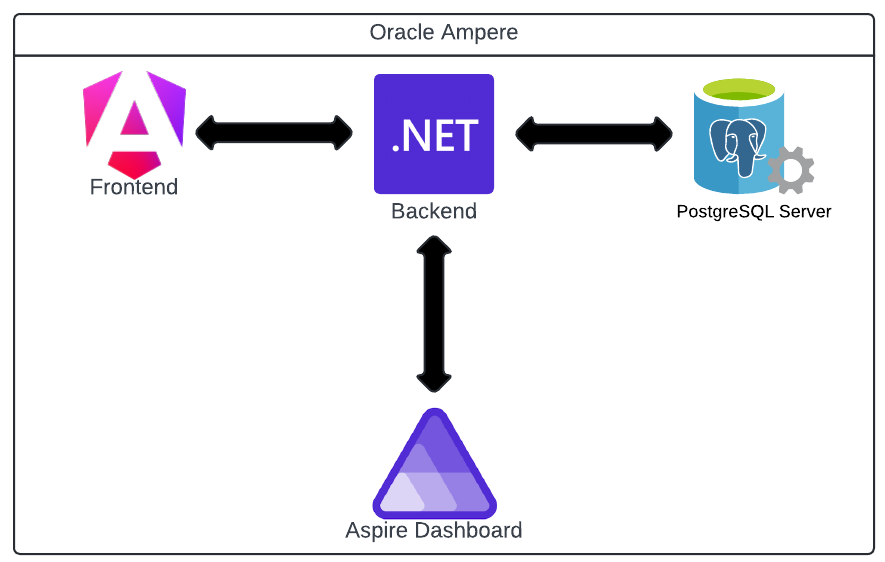
\includegraphics[width=1\textwidth]{attachments/arch-diag}
    \caption{Diagram systemu w środowisku docelowym}
    \label{fig:figure}
\end{figure}

\pagebreak
\subsection{Konfiguracja Nginx}
\label{subsec:konfiguracja-nginx}
Przedstawiona poniżej konfiguracja serwera NGINX zawiera definicje kilku serwerów wirtualnych dla różnych domen i usług.
Zamieszczono w niej szczegółowe wyjaśnienie każdego elementu konfiguracji.

\subsubsection{Główny serwer obsługujący \texttt{city-planner.budziszm.pl}}
\begin{longlisting}[language=nginx,label={lst:n1}]
server {
  server_name city-planner.budziszm.pl;

  root /var/www/city-planner.budziszm.pl/html;

  index index.html;
\end{longlisting}
\begin{itemize}
    \item \texttt{server\_name city-planner.budziszm.pl;}: Określa nazwę serwera, który obsługuje tę konfigurację.
    \item \texttt{root /var/www/city-planner.budziszm.pl/html;}: Ustala katalog główny dla plików serwowanych przez ten serwer.
    \item \texttt{index index.html;}: Ustawia domyślny plik indeksu.
\end{itemize}

\begin{longlisting}[language=nginx,label={lst:n2}]
  location = /favicon.ico { access_log off; log_not_found off; }
\end{longlisting}
\begin{itemize}
    \item \texttt{location = /favicon.ico}: Reguła dla \texttt{favicon.ico}.
    Wyłącza logowanie dostępu oraz błędów, jeśli plik nie zostanie znaleziony.
\end{itemize}

\subsubsection{Konfiguracja gzip}
\begin{longlisting}[language=nginx,label={lst:n3}]
  gzip on;
  gzip_static on;
  gzip_types
    text/plain
    text/css
    text/js
    text/xml
    text/javascript
    application/javascript
    application/json
    application/xml
    application/rss+xml
    image/svg+xml;
  gzip_proxied no-cache no-store private expired auth;
\end{longlisting}
\begin{itemize}
    \item \texttt{gzip on;} i \texttt{gzip\_static on;}: Włącza kompresję gzip i kompresję statyczną.
    \item \texttt{gzip\_types}: Określa typy MIME, które mają być kompresowane.
    \item \texttt{gzip\_proxied}: Definiuje warunki, pod którymi odpowiedzi z proxy mogą być kompresowane.
\end{itemize}

\subsubsection{Konfiguracja cache dla CSS i JS}
\begin{longlisting}[language=nginx,label={lst:n4}]
  location ~*.(css|js)$ {
    add_header Cache-Control "public, immutable, max-age=31536000";
  }
\end{longlisting}
\begin{itemize}
    \item \texttt{location ~*.(css|js)\$}: Obsługuje wszystkie pliki CSS i JS@.
    \item \texttt{add\_header Cache-Control "public, immutable, max-age=31536000";}: Dodaje nagłówek kontrolujący cache, który umożliwia przechowywanie plików w pamięci podręcznej przez rok.
\end{itemize}

\subsubsection{Przekierowania proxy dla \texttt{/Api} i \texttt{/confirmEmail}}
\begin{longlisting}[language=nginx,label={lst:n5}]
  location /Api {
    rewrite /Api/(.*) /$1 break;
    proxy_pass http://localhost:5000;
    proxy_redirect off;
    proxy_set_header Host $host;
  }

  location /confirmEmail {
    proxy_pass http://localhost:5000;
    proxy_redirect off;
    proxy_set_header Host $host;
  }
\end{longlisting}
\begin{itemize}
    \item \texttt{location /Api} i \texttt{location /confirmEmail}: Przekierowują żądania na odpowiednie endpointy do lokalnego serwera działającego na porcie 5000.
\end{itemize}

\subsubsection{Obsługa plików w \texttt{/thesis}}
\begin{longlisting}[language=nginx,label={lst:n6}]
  location ~* /thesis/(.*)$ {
    root /opt/city-planner-documentation;
    rewrite /thesis/(.*) /$1.pdf break;
    add_header Content-Disposition 'inline';
    try_files $uri =404;
  }

  location /thesis {
    root /opt/city-planner-documentation;
    rewrite /thesis /thesis.pdf break;
    add_header Content-Disposition 'inline';
    try_files $uri =404;
  }
\end{longlisting}
\begin{itemize}
    \item Obsługuje dostęp do plików w katalogu \texttt{/opt/city-planner-documentation}, zmieniając ścieżki i dodając nagłówek \texttt{Content-Disposition} do wyświetlania plików PDF w przeglądarce.
\end{itemize}

\subsubsection{Główne ustawienia dla ścieżek i SSL}
\begin{longlisting}[language=nginx,label={lst:n7}]
  location / {
    try_files $uri$args $uri$args/ /index.html;
  }

  listen 443 ssl; # managed by Certbot
  ssl_certificate /etc/letsencrypt/live/city-planner.budziszm.pl/fullchain.pem; # managed by Certbot
  ssl_certificate_key /etc/letsencrypt/live/city-planner.budziszm.pl/privkey.pem; # managed by Certbot
  include /etc/letsencrypt/options-ssl-nginx.conf; # managed by Certbot
  ssl_dhparam /etc/letsencrypt/ssl-dhparams.pem; # managed by Certbot
\end{longlisting}
\begin{itemize}
    \item \texttt{location /}: Przekierowuje do pliku \texttt{index.html} jeśli plik lub katalog nie zostaną znalezione.
    \item \texttt{listen 443 ssl;}: Konfiguruje serwer do nasłuchiwania na porcie 443 z SSL\@.
    \item \texttt{ssl\_certificate}, \texttt{ssl\_certificate\_key}, \texttt{include}, \texttt{ssl\_dhparam}: Konfiguracja SSL przy użyciu certyfikatów Let's Encrypt.
\end{itemize}

\subsubsection{Przekierowanie HTTP do HTTPS}
\begin{longlisting}[language=nginx,label={lst:n8}]
server {
    if ($host = city-planner.budziszm.pl) {
        return 301 https://$host$request_uri;
    } # managed by Certbot

    server_name city-planner.budziszm.pl;
    listen 80;
    return 404; # managed by Certbot
}
\end{longlisting}
\begin{itemize}
    \item Przekierowuje ruch HTTP na HTTPS dla \texttt{city-planner.budziszm.pl}.
\end{itemize}

\subsubsection{Serwer obsługujący \texttt{logs.city-planner.budziszm.pl}}
\begin{longlisting}[language=nginx,label={lst:n9}]
server {
  server_name logs.city-planner.budziszm.pl;
  auth_basic           "Administrator's Area";
  auth_basic_user_file /etc/apache2/.htpasswd;
  error_log  /var/log/nginx/error.log debug;

  location / {
    proxy_pass https://localhost:18888;
    proxy_redirect off;
    proxy_http_version 1.1;
    proxy_set_header Upgrade $http_upgrade;
    proxy_set_header Connection "Upgrade";
    proxy_set_header Host $host;
  }

  listen 443 ssl; # managed by Certbot
  ssl_certificate /etc/letsencrypt/live/city-planner.budziszm.pl/fullchain.pem; # managed by Certbot
  ssl_certificate_key /etc/letsencrypt/live/city-planner.budziszm.pl/privkey.pem; # managed by Certbot
  include /etc/letsencrypt/options-ssl-nginx.conf; # managed by Certbot
  ssl_dhparam /etc/letsencrypt/ssl-dhparams.pem; # managed by Certbot
}
\end{longlisting}
\begin{itemize}
    \item Obsługuje ruch na \texttt{logs.city-planner.budziszm.pl} z podstawową autoryzacją.
    \item Przekierowuje ruch do lokalnego serwera na porcie 18888 z obsługą WebSocketów.
\end{itemize}

\subsubsection{Przekierowanie HTTP do HTTPS dla \texttt{logs.city-planner.budziszm.pl}}
\begin{longlisting}[language=nginx,label={lst:n10}]
server {
    if ($host = logs.city-planner.budziszm.pl) {
        return 301 https://$host$request_uri;
    } # managed by Certbot

    listen 80;
    server_name logs.city-planner.budziszm.pl;
    return 404; # managed by Certbot
}
\end{longlisting}
\begin{itemize}
    \item Przekierowuje ruch HTTP na HTTPS dla \texttt{logs.city-planner.budziszm.pl}.
\end{itemize}

\subsubsection{Mapowanie nagłówka \texttt{Connection} w zależności od nagłówka \texttt{Upgrade}}
\begin{longlisting}[language=nginx,label={lst:n11}]
map $http_upgrade $connection_upgrade {
  default upgrade;
  ''      close;
}
\end{longlisting}
\begin{itemize}
    \item Ustawia wartość nagłówka \texttt{Connection} w zależności od obecności nagłówka \texttt{Upgrade}.
    Umożliwia to poprawne działanie WebSocketów.
\end{itemize}

Ta konfiguracja zapewnia pełną obsługę zarówno dla serwowania statycznych stron, jak i przekierowania ruchu do usług backendowych, zapewniając jednocześnie bezpieczeństwo przez użycie SSL i kontrolę cache dla plików statycznych.

\subsection{Deployment backendu}
\label{subsec:deployment-backendu}
Ten skrypt Bash wykonuje kilka kroków, aby wdrożyć backend aplikacji.
Poniżej znajduje się szczegółowy opis, co robi każda jego część:

\subsubsection{Usuwanie wszystkich plików z /opt/city-planner-backend/publish}
Ten krok usuwa wszystkie pliki z katalogu \texttt{/opt/city-planner-backend/publish}, aby przygotować miejsce na nowe pliki.
\begin{longlisting}[style=shell-colored,label={lst:db1}]
+echo+ "Removing all files from /opt/city-planner-backend/publish"
+rm -Rf+ /opt/city-planner-backend/publish/*
\end{longlisting}

\subsubsection{Kopiowanie plików do /opt/city-planner-backend/publish/}
Ten krok kopiuje opublikowane pliki z katalogu \texttt{WebApi/bin/production/net8.0/linux-arm64/publish/} do \texttt{/opt/city-planner-backend/publish/}.
\begin{longlisting}[style=shell-colored,label={lst:db2}]
+echo+ "Copying publish files to /opt/city-planner-backend/publish/"
+cp+ WebApi/bin/production/net8.0/linux-arm64/publish/* /opt/city-planner-backend/publish/
\end{longlisting}

\subsubsection{Przygotowanie pliku usługi SystemD}
Ten krok tworzy nowy plik usługi SystemD dla backendu aplikacji.
Plik usługi zawiera konfigurację dla SystemD, w tym opis, zależności, ustawienia serwisu i polecenie uruchomienia.

\begin{longlisting}[style=shell-colored,label={lst:db3}]
+echo+ "Preparing SystemD service file"
+rm -f+ /etc/systemd/system/city-planner-backend.service
+cat+ <<EOT >> /etc/systemd/system/city-planner-backend.service
[Unit]
Description=City planner backend
After=network.target
StartLimitIntervalSec=0

[Service]
Type=simple
Restart=always
RestartSec=1
User=ubuntu
EnvironmentFile=/opt/city-planner-backend/environment.conf
WorkingDirectory=/opt/city-planner-backend/publish
ExecStart=/opt/city-planner-backend/publish/WebApi

[Install]
WantedBy=multi-user.target
EOT
\end{longlisting}

\subsubsection{Włączanie pliku usługi SystemD}
Ten krok włącza nowo utworzony plik usługi SystemD, aby uruchamiał się automatycznie przy starcie systemu.
\begin{longlisting}[style=shell-colored,label={lst:db4}]
+echo+ "Enabling SystemD service file"
+systemctl enable+ city-planner-backend
\end{longlisting}

\subsubsection{Restartowanie usługi SystemD}
Ten krok restartuje usługę SystemD, aby zastosować nowe ustawienia i uruchomić backend aplikacji.
\begin{longlisting}[style=shell-colored,label={lst:db5}]
+echo+ "Restarting SystemD service file"
+systemctl restart+ city-planner-backend
\end{longlisting}

\subsubsection{Zakończenie wdrożenia backendu}
Ten krok wyświetla komunikat informujący o zakończeniu wdrożenia backendu.
\begin{longlisting}[style=shell-colored,label={lst:db6}]
+echo+ "Backend deployment done"
\end{longlisting}

\subsubsection{Całość kodu}
\begin{longlisting}[style=shell-colored,label={lst:db7}]
#!/bin/bash

+echo+ "Removing all files from /opt/city-planner-backend/publish"
+rm -Rf+ /opt/city-planner-backend/publish/*

+echo+ "Copying publish files to /opt/city-planner-backend/publish/"
+cp+ WebApi/bin/production/net8.0/linux-arm64/publish/* /opt/city-planner-backend/publish/
+echo+ "Preparing SystemD service file"
+rm -f+ /etc/systemd/system/city-planner-backend.service
+cat+ <<EOT >> /etc/systemd/system/city-planner-backend.service
[Unit]
Description=City planner backend
After=network.target
StartLimitIntervalSec=0

[Service]
Type=simple
Restart=always
RestartSec=1
User=ubuntu
EnvironmentFile=/opt/city-planner-backend/environment.conf
WorkingDirectory=/opt/city-planner-backend/publish
ExecStart=/opt/city-planner-backend/publish/WebApi

[Install]
WantedBy=multi-user.target
EOT

+echo+ "Enabling SystemD service file"
+systemctl enable+ city-planner-backend
+echo+ "Restarting SystemD service file"
+systemctl restart+ city-planner-backend

+echo+ "Backend deployment done"
\end{longlisting}

\subsection{Deployment frontendu}
Ten skrypt Bash wykonuje kilka kroków, aby wdrożyć frontend aplikacji.
Poniżej znajduje się szczegółowy opis, co robi każda jego część:

\subsubsection{Usuwanie wszystkich plików z \newline
/var/www/city-planner.budziszm.pl/html}
Ten krok usuwa wszystkie pliki z katalogu \texttt{/var/www/city-planner.budziszm.pl/html}, aby przygotować miejsce na nowe pliki.
\begin{longlisting}[style=shell-colored]
+echo+ "Removing all files from /var/www/city-planner.budziszm.pl/html"
+rm -Rf+ /var/www/city-planner.budziszm.pl/html/*
\end{longlisting}

\subsubsection{Kopiowanie plików do /var/www/city-planner.budziszm.pl/html/}
Ten krok kopiuje pliki z katalogu \texttt{dist/frontend/browser/} \newline
do \texttt{/var/www/city-planner.budziszm.pl/html/}.
\begin{longlisting}[style=shell-colored]
+echo+ "Copying dist files to /var/www/city-planner.budziszm.pl/html/"
+cp -r+ dist/frontend/browser/* /var/www/city-planner.budziszm.pl/html/
\end{longlisting}

\subsubsection{Zakończenie wdrożenia frontendu}
Ten krok wyświetla komunikat informujący o zakończeniu wdrożenia frontendu.
\begin{longlisting}[style=shell-colored]
+echo+ "Frontend deployment done"
\end{longlisting}

\subsubsection{Całość kodu}
\begin{longlisting}[style=shell-colored]
#!/bin/bash

+echo+ "Removing all files from /var/www/city-planner.budziszm.pl/html"
+rm -Rf+ /var/www/city-planner.budziszm.pl/html/*

+echo+ "Copying dist files to /var/www/city-planner.budziszm.pl/html/"
+cp -r+ dist/frontend/browser/* /var/www/city-planner.budziszm.pl/html/

+echo+ "Frontend deployment done"
\end{longlisting}

\section{Specyfikacja API}
Do implementacji API został użyty framework ASP.NET, który umożliwia tworzenie wydajnych i skalowalnych aplikacji webowych. Do zarządzania warstwą dostępu do danych i mapowania obiektowo-relacyjnego (ORM) zastosowano Entity Framework, w połączeniu z biblioteką Npgsql, która pozwala na efektywną współpracę z bazą danych PostgreSQL\@.
Dzięki temu rozwiązaniu możliwe było stworzenie solidnej i wydajnej aplikacji z wykorzystaniem nowoczesnych technologii .NET, zapewniając jednocześnie łatwość w zarządzaniu danymi i wysoką kompatybilność z relacyjnymi bazami danych.

W trakcie prac do prezentacji dokumentacji endpointów użyto Swaggera i ReDoca.

\begin{figure}[H]
\centering
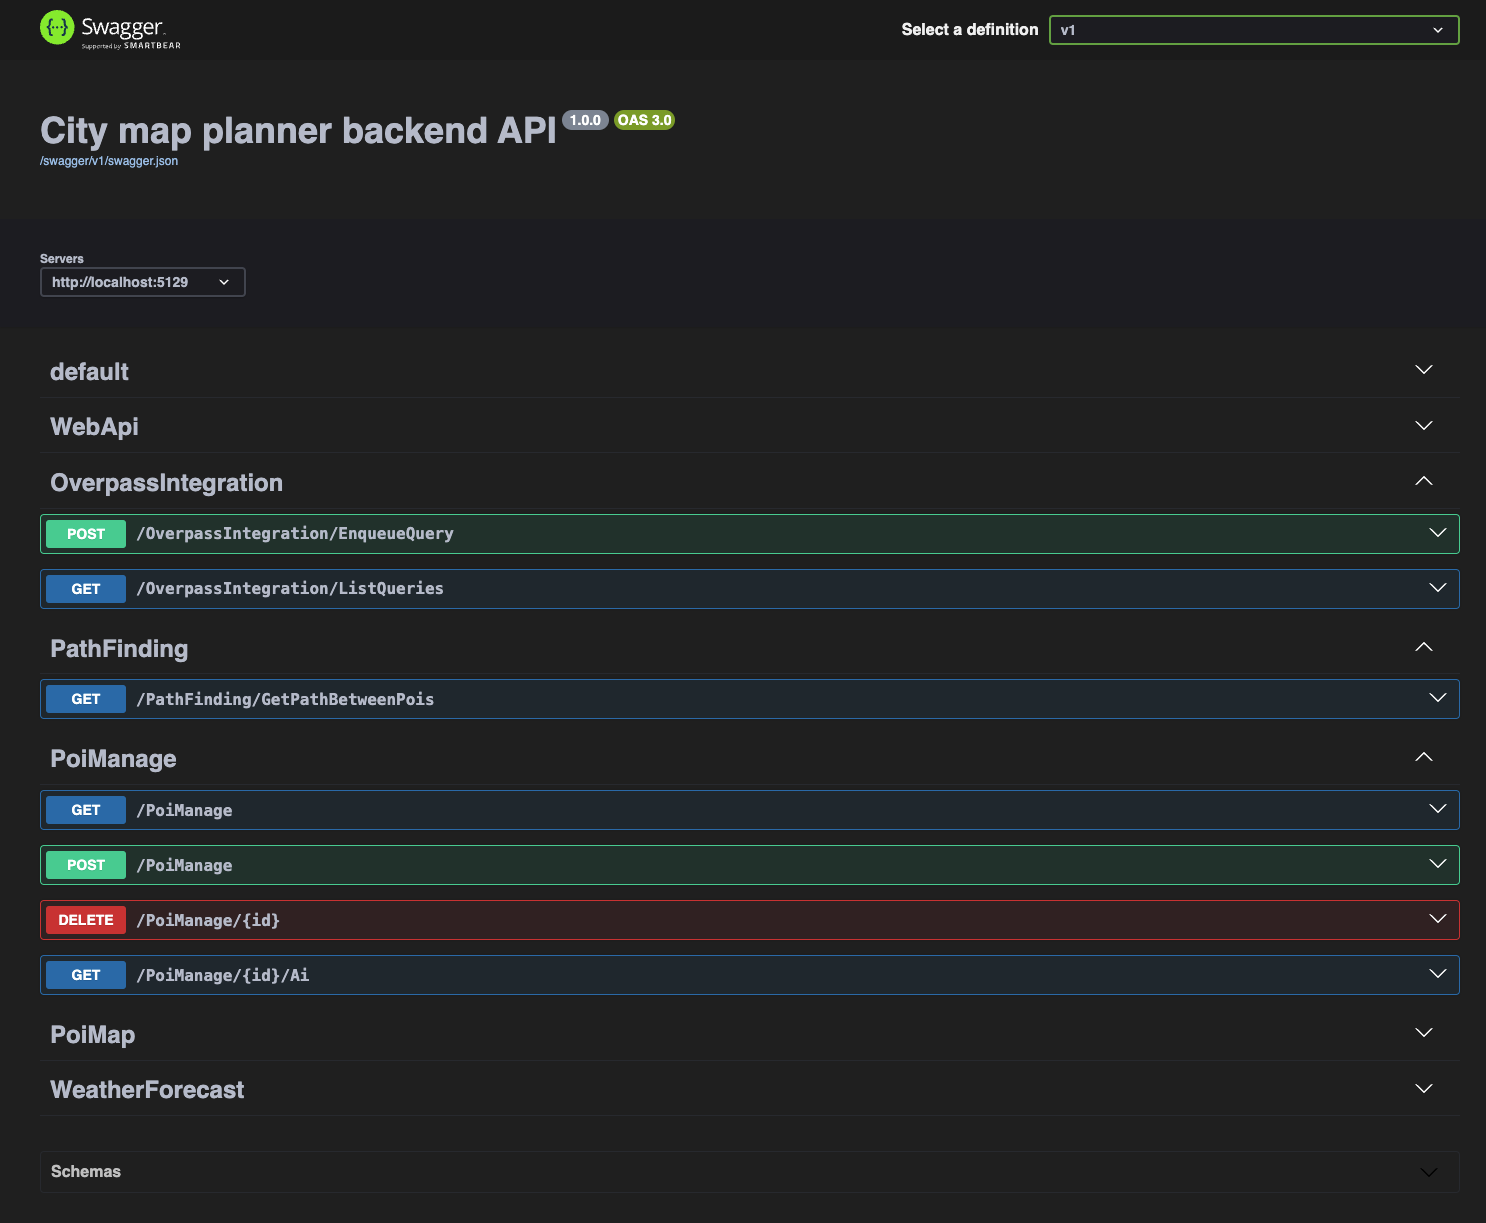
\includegraphics[width=1\textwidth]{attachments/swagger}
\caption{Dokumentacji API w programie Swagger}
\label{fig:figure}
\end{figure}

\begin{figure}[H]
\centering

\includegraphics[width=1\textwidth]{attachments/redoc}
\caption{Dokumentacji API w programie ReDoc}
\label{fig:figure}
\end{figure}

Poniżej przedstawiono specyfikację dostępnych punktów końcowych:

\subsection{Autoryzacja i zarządzanie użytkownikami}
\subsubsection{\lstinline[language=http]{POST /register}}
Rejestracja nowego użytkownika. \\
\textbf{Request body:}
\begin{lstlisting}[language=json]
{
  "email": "string",
  "password": "string"
}
\end{lstlisting}
\textbf{Responses:}
\begin{itemize}
    \item 200: Rejestracja powiodła się.
    \item 400: Błąd walidacji danych.
\begin{lstlisting}[language=json]
{
  "type": "string",
  "title": "string",
  "status": 0,
  "detail": "string",
  "instance": "string",
  "errors": {
    "additionalProp1": [
      "string"
    ],
    "additionalProp2": [
      "string"
    ],
    "additionalProp3": [
      "string"
    ]
  }
}
\end{lstlisting}
\end{itemize}

\subsubsection{\lstinline[language=http]{POST /login}}
Logowanie użytkownika. \\
\textbf{Query parameters:}
\begin{itemize}
    \item \texttt{useCookies} (boolean, opcjonalny)
    \item \texttt{useSessionCookies} (boolean, opcjonalny)
\end{itemize}
\textbf{Request body:}
\begin{lstlisting}[language=json]
{
  "email": "string",
  "password": "string",
  "twoFactorCode": "string",
  "twoFactorRecoveryCode": "string"
}
\end{lstlisting}
\textbf{Responses:}
\begin{itemize}
    \item 200:
\begin{lstlisting}[language=json]
{
  "tokenType": "string",
  "accessToken": "string",
  "expiresIn": 0,
  "refreshToken": "string"
}
\end{lstlisting}
\end{itemize}

\subsubsection{\lstinline[language=http]{POST /refresh}}
Odświeżenie tokenu autoryzacyjnego. \\
\textbf{Request body:}
\begin{lstlisting}[language=json]
{
  "refreshToken": "string"
}
\end{lstlisting}
\textbf{Responses:}
\begin{itemize}
    \item 200:
\begin{lstlisting}[language=json]
{
  "tokenType": "string",
  "accessToken": "string",
  "expiresIn": 0,
  "refreshToken": "string"
}
\end{lstlisting}
\end{itemize}

\subsubsection{\lstinline[language=http]{GET /confirmEmail}}
Potwierdzenie adresu email. \\
\textbf{Query parameters:}
\begin{itemize}
    \item \texttt{userId} (string, opcjonalny)
    \item \texttt{code} (string, opcjonalny)
    \item \texttt{changedEmail} (string, opcjonalny)
\end{itemize}
\textbf{Responses:}
\begin{itemize}
    \item 200: Potwierdzenie zakończone sukcesem.
\end{itemize}

\subsubsection{\lstinline[language=http]{POST /resendConfirmationEmail}}
Ponowne wysłanie emaila z potwierdzeniem. \\
\textbf{Request body:}
\begin{lstlisting}[language=json]
{
  "email": "string"
}
\end{lstlisting}
\textbf{Responses:}
\begin{itemize}
    \item 200: Email z potwierdzeniem wysłany ponownie.
\end{itemize}

\subsubsection{\lstinline[language=http]{POST /forgotPassword}}
Przypomnienie hasła. \\
\textbf{Request body:}
\begin{lstlisting}[language=json]
{
  "email": "string"
}
\end{lstlisting}
\textbf{Responses:}
\begin{itemize}
    \item 200: Email z instrukcjami wysłany.
    \item 400:
\begin{lstlisting}[language=json]
{
  "type": "string",
  "title": "string",
  "status": 0,
  "detail": "string",
  "instance": "string",
  "errors": {
    "additionalProp1": [
      "string"
    ],
    "additionalProp2": [
      "string"
    ],
    "additionalProp3": [
      "string"
    ]
  }
}
\end{lstlisting}
\end{itemize}

\subsubsection{\lstinline[language=http]{POST /resetPassword}}
Resetowanie hasła. \\
\textbf{Request body:}
\begin{lstlisting}[language=json]
{
  "email": "string",
  "resetCode": "string",
  "newPassword": "string"
}
\end{lstlisting}
\textbf{Responses:}
\begin{itemize}
    \item 200: Hasło zresetowane.
    \item 400:
\begin{lstlisting}[language=json]
{
  "type": "string",
  "title": "string",
  "status": 0,
  "detail": "string",
  "instance": "string",
  "errors": {
    "additionalProp1": [
      "string"
    ],
    "additionalProp2": [
      "string"
    ],
    "additionalProp3": [
      "string"
    ]
  }
}
\end{lstlisting}
\end{itemize}

\subsubsection{\lstinline[language=http]{POST /manage/2fa}}
Zarządzanie dwuskładnikowym uwierzytelnianiem (2FA). \\
\textbf{Request body:}
\begin{lstlisting}[language=json]
{
  "enable": true,
  "twoFactorCode": "string",
  "resetSharedKey": true,
  "resetRecoveryCodes": true,
  "forgetMachine": true
}
\end{lstlisting}
\textbf{Responses:}
\begin{itemize}
    \item 200:
\begin{lstlisting}[language=json]
{
  "sharedKey": "string",
  "recoveryCodesLeft": 0,
  "recoveryCodes": [
    "string"
  ],
  "isTwoFactorEnabled": true,
  "isMachineRemembered": true
}
\end{lstlisting}
    \item 400:
\begin{lstlisting}[language=json]
{
  "type": "string",
  "title": "string",
  "status": 0,
  "detail": "string",
  "instance": "string",
  "errors": {
    "additionalProp1": [
      "string"
    ],
    "additionalProp2": [
      "string"
    ],
    "additionalProp3": [
      "string"
    ]
  }
}
\end{lstlisting}
    \item 404: Nie znaleziono zasobu.
\end{itemize}

\subsubsection{\lstinline[language=http]{GET /manage/info}}
Pobranie informacji o koncie. \\
\textbf{Responses:}
\begin{itemize}
    \item 200:
\begin{lstlisting}[language=json]
{
  "email": "string",
  "isEmailConfirmed": true
}
\end{lstlisting}
    \item 400:
\begin{lstlisting}[language=json]
{
  "type": "string",
  "title": "string",
  "status": 0,
  "detail": "string",
  "instance": "string",
  "errors": {
    "additionalProp1": [
      "string"
    ],
    "additionalProp2": [
      "string"
    ],
    "additionalProp3": [
      "string"
    ]
  }
}
\end{lstlisting}
    \item 404: Nie znaleziono zasobu.
\end{itemize}

\subsubsection{\lstinline[language=http]{POST /manage/info}}
Aktualizacja informacji o koncie. \\
\textbf{Request body:}
\begin{lstlisting}[language=json]
{
  "newEmail": "string",
  "newPassword": "string",
  "oldPassword": "string"
}
\end{lstlisting}
\textbf{Responses:}
\begin{itemize}
    \item 200:
\begin{lstlisting}[language=json]
{
  "email": "string",
  "isEmailConfirmed": true
}
\end{lstlisting}
    \item 400:
\begin{lstlisting}[language=json]
{
  "type": "string",
  "title": "string",
  "status": 0,
  "detail": "string",
  "instance": "string",
  "errors": {
    "additionalProp1": [
      "string"
    ],
    "additionalProp2": [
      "string"
    ],
    "additionalProp3": [
      "string"
    ]
  }
}
\end{lstlisting}
    \item 404: Nie znaleziono zasobu.
\end{itemize}

\subsubsection{\lstinline[language=http]{POST /logout}}
Wylogowanie użytkownika. \\
\textbf{Request body:} Pusty JSON \\
\textbf{Responses:}
\begin{itemize}
    \item 200: Wylogowanie zakończone sukcesem.
\end{itemize}

\subsubsection{\lstinline[language=http]{GET /exists}}
Sprawdzenie czy email istnieje w systemie. \\
\textbf{Query parameters:}
\begin{itemize}
    \item \texttt{email} (string, wymagany)
\end{itemize}
\textbf{Responses:}
\begin{itemize}
    \item 200: Email istnieje.
\end{itemize}

\subsubsection{\lstinline[language=http]{POST /deleteMe}}
Usunięcie konta użytkownika. \\
\textbf{Responses:}
\begin{itemize}
    \item 200: Konto usunięte.
\end{itemize}

\subsection{Integracja z Overpass}

\subsubsection{\lstinline[language=http]{POST /OverpassIntegration/EnqueueQuery}}
Kolejkowanie zapytania Overpass. \\
\textbf{Responses:}
\begin{itemize}
    \item 200: Zapytanie dodane do kolejki.
\end{itemize}

\subsubsection{\lstinline[language=http]{GET /OverpassIntegration/ListQueries}}
Pobranie listy zapytań Overpass. \\
\textbf{Responses:}
\begin{lstlisting}[language=json]
[
  "string"
]
\end{lstlisting}
\begin{itemize}
    \item 401: Nieautoryzowany dostęp.
\end{itemize}

\subsection{Zarządzanie Punktami POI}

\subsubsection{\lstinline[language=http]{GET /PoiManage}}
Pobranie listy punktów POI. \\
\textbf{Responses:}
\begin{lstlisting}[language=json]
[
  {
    "id": 0,
    "name": "string",
    "description": "string",
    "modified": "2023-01-01T00:00:00Z",
    "businessHoursPageUrl": "string",
    "businessHoursPageXPath": "string",
    "businessHoursPageModified": "2023-01-01T00:00:00Z",
    "holidaysPageUrl": "string",
    "holidaysPageXPath": "string",
    "holidaysPageModified": "2023-01-01T00:00:00Z",
    "entrances": [
      {
        "osmNodeId": 0,
        "name": "string",
        "description": "string"
      }
    ],
    "images": [
      {
        "fullSrc": "string",
        "iconSrc": "string",
        "attribution": "string"
      }
    ],
    "preferredWmoCodes": [
      0
    ],
    "preferredSightseeingTime": "string",
    "businessTimes": [
      {
        "effectiveFrom": "2023-01-01T00:00:00Z",
        "effectiveTo": "2023-01-01T00:00:00Z",
        "effectiveDays": [
          0
        ],
        "timeFrom": "00:00:00",
        "timeTo": "00:00:00",
        "state": 0
      }
    ]
  }
]
\end{lstlisting}

\subsubsection{\lstinline[language=http]{POST /PoiManage}}
Dodanie lub aktualizacja punktu POI. \\
\textbf{Request body:}
\begin{lstlisting}[language=json]
{
  "id": 0,
  "name": "string",
  "description": "string",
  "modified": "2023-01-01T00:00:00Z",
  "businessHoursPageUrl": "string",
  "businessHoursPageXPath": "string",
  "businessHoursPageModified": "2023-01-01T00:00:00Z",
  "holidaysPageUrl": "string",
  "holidaysPageXPath": "string",
  "holidaysPageModified": "2023-01-01T00:00:00Z",
  "entrances": [
    {
      "osmNodeId": 0,
      "name": "string",
      "description": "string"
    }
  ],
  "images": [
    {
      "fullSrc": "string",
      "iconSrc": "string",
      "attribution": "string"
    }
  ],
  "preferredWmoCodes": [
    0
  ],
  "preferredSightseeingTime": "string",
  "businessTimes": [
    {
      "effectiveFrom": "2023-01-01T00:00:00Z",
      "effectiveTo": "2023-01-01T00:00:00Z",
      "effectiveDays": [
        0
      ],
      "timeFrom": "00:00:00",
      "timeTo": "00:00:00",
      "state": 0
    }
  ]
}
\end{lstlisting}
\textbf{Responses:}
\begin{lstlisting}[language=json]
{
  "id": 0,
  "name": "string",
  "description": "string",
  "modified": "2023-01-01T00:00:00Z",
  "businessHoursPageUrl": "string",
  "businessHoursPageXPath": "string",
  "businessHoursPageModified": "2023-01-01T00:00:00Z",
  "holidaysPageUrl": "string",
  "holidaysPageXPath": "string",
  "holidaysPageModified": "2023-01-01T00:00:00Z",
  "entrances": [
    {
      "osmNodeId": 0,
      "name": "string",
      "description": "string"
    }
  ],
  "images": [
    {
      "fullSrc": "string",
      "iconSrc": "string",
      "attribution": "string"
    }
  ],
  "preferredWmoCodes": [
    0
  ],
  "preferredSightseeingTime": "string",
  "businessTimes": [
    {
      "effectiveFrom": "2023-01-01T00:00:00Z",
      "effectiveTo": "2023-01-01T00:00:00Z",
      "effectiveDays": [
        0
      ],
      "timeFrom": "00:00:00",
      "timeTo": "00:00:00",
      "state": 0
    }
  ]
}
\end{lstlisting}

\subsubsection{\lstinline[language=http]{DELETE /PoiManage/\{id\}}}
Usunięcie punktu POI. \\
\textbf{Path parameters:}
\begin{itemize}
    \item \texttt{id} (integer, wymagany)
\end{itemize}
\textbf{Responses:}
\begin{itemize}
    \item 200: Punkt POI usunięty.
\end{itemize}

\subsubsection{\lstinline[language=http]{GET /PoiManage/\{id\}/Ai}}
Pobranie informacji AI dla punktu POI. \\
\textbf{Path parameters:}
\begin{itemize}
    \item \texttt{id} (integer, wymagany)
\end{itemize}
\textbf{Responses:}
\begin{lstlisting}[language=json]
[
  {
    "effectiveFrom": "2023-01-01T00:00:00Z",
    "effectiveTo": "2023-01-01T00:00:00Z",
    "effectiveDays": [
      0
    ],
    "timeFrom": "00:00:00",
    "timeTo": "00:00:00",
    "state": 0
  }
]
\end{lstlisting}

\subsection{Mapowanie Punktów POI}

\subsubsection{\lstinline[language=http]{GET /PoiMap/List}}
Lista punktów POI na mapie. \\
\textbf{Responses:}
\begin{lstlisting}[language=json]
[
  {
    "id": 0,
    "map": {
      "label": "string",
      "iconSrc": "string",
      "lat": 0,
      "lon": 0
    },
    "details": {
      "bannerSrc": "string",
      "title": "string",
      "description": "string"
    },
    "preferredSightseeingTime": "string",
    "businessHours": [
      {
        "effectiveFrom": "2023-01-01T00:00:00Z",
        "effectiveTo": "2023-01-01T00:00:00Z",
        "effectiveDays": [
          0
        ],
        "timeFrom": "00:00:00",
        "timeTo": "00:00:00",
        "state": 0
      }
    ]
  }
]
\end{lstlisting}

\subsubsection{\lstinline[language=http]{GET /WeatherForecast}}
Pobranie prognozy pogody. \\
\textbf{Responses:}
\begin{lstlisting}[language=json]
[
  {
    "date": "2023-01-01",
    "temperatureC": 0,
    "temperatureF": 0,
    "summary": "string"
  }
]
\end{lstlisting}

	%! Author = Mateusz Budzisz
%! Date = 26/05/2024

\chapter{Realizacja Projektu}
\label{ch:realizacja}
Po zakończeniu prac analitycznych i omówieniu przewidywanych funkcjonalności przeprowadzono analizę możliwych decyzji projektowych. Podjęto działania umożliwiające wybór odpowiednich rozwiązań projektowych. 
Następnie przystąpiono do realizacji poszczególnych komponentów systemu.

\section{Aplikacja City Map Planner}
\label{sec:aplikacja}

\subsection{Przyrost I - utworzenie szkieletu aplikacji oraz Potoki testów aplikacji}
\label{sec:przyrost1}

W ramach tego przyrostu pierwszego wykonano:
\begin{itemize}
    \item backend WebAPI z podstawowym testem działania funkcjonowania;
    \begin{figure}[H]
        \centering
        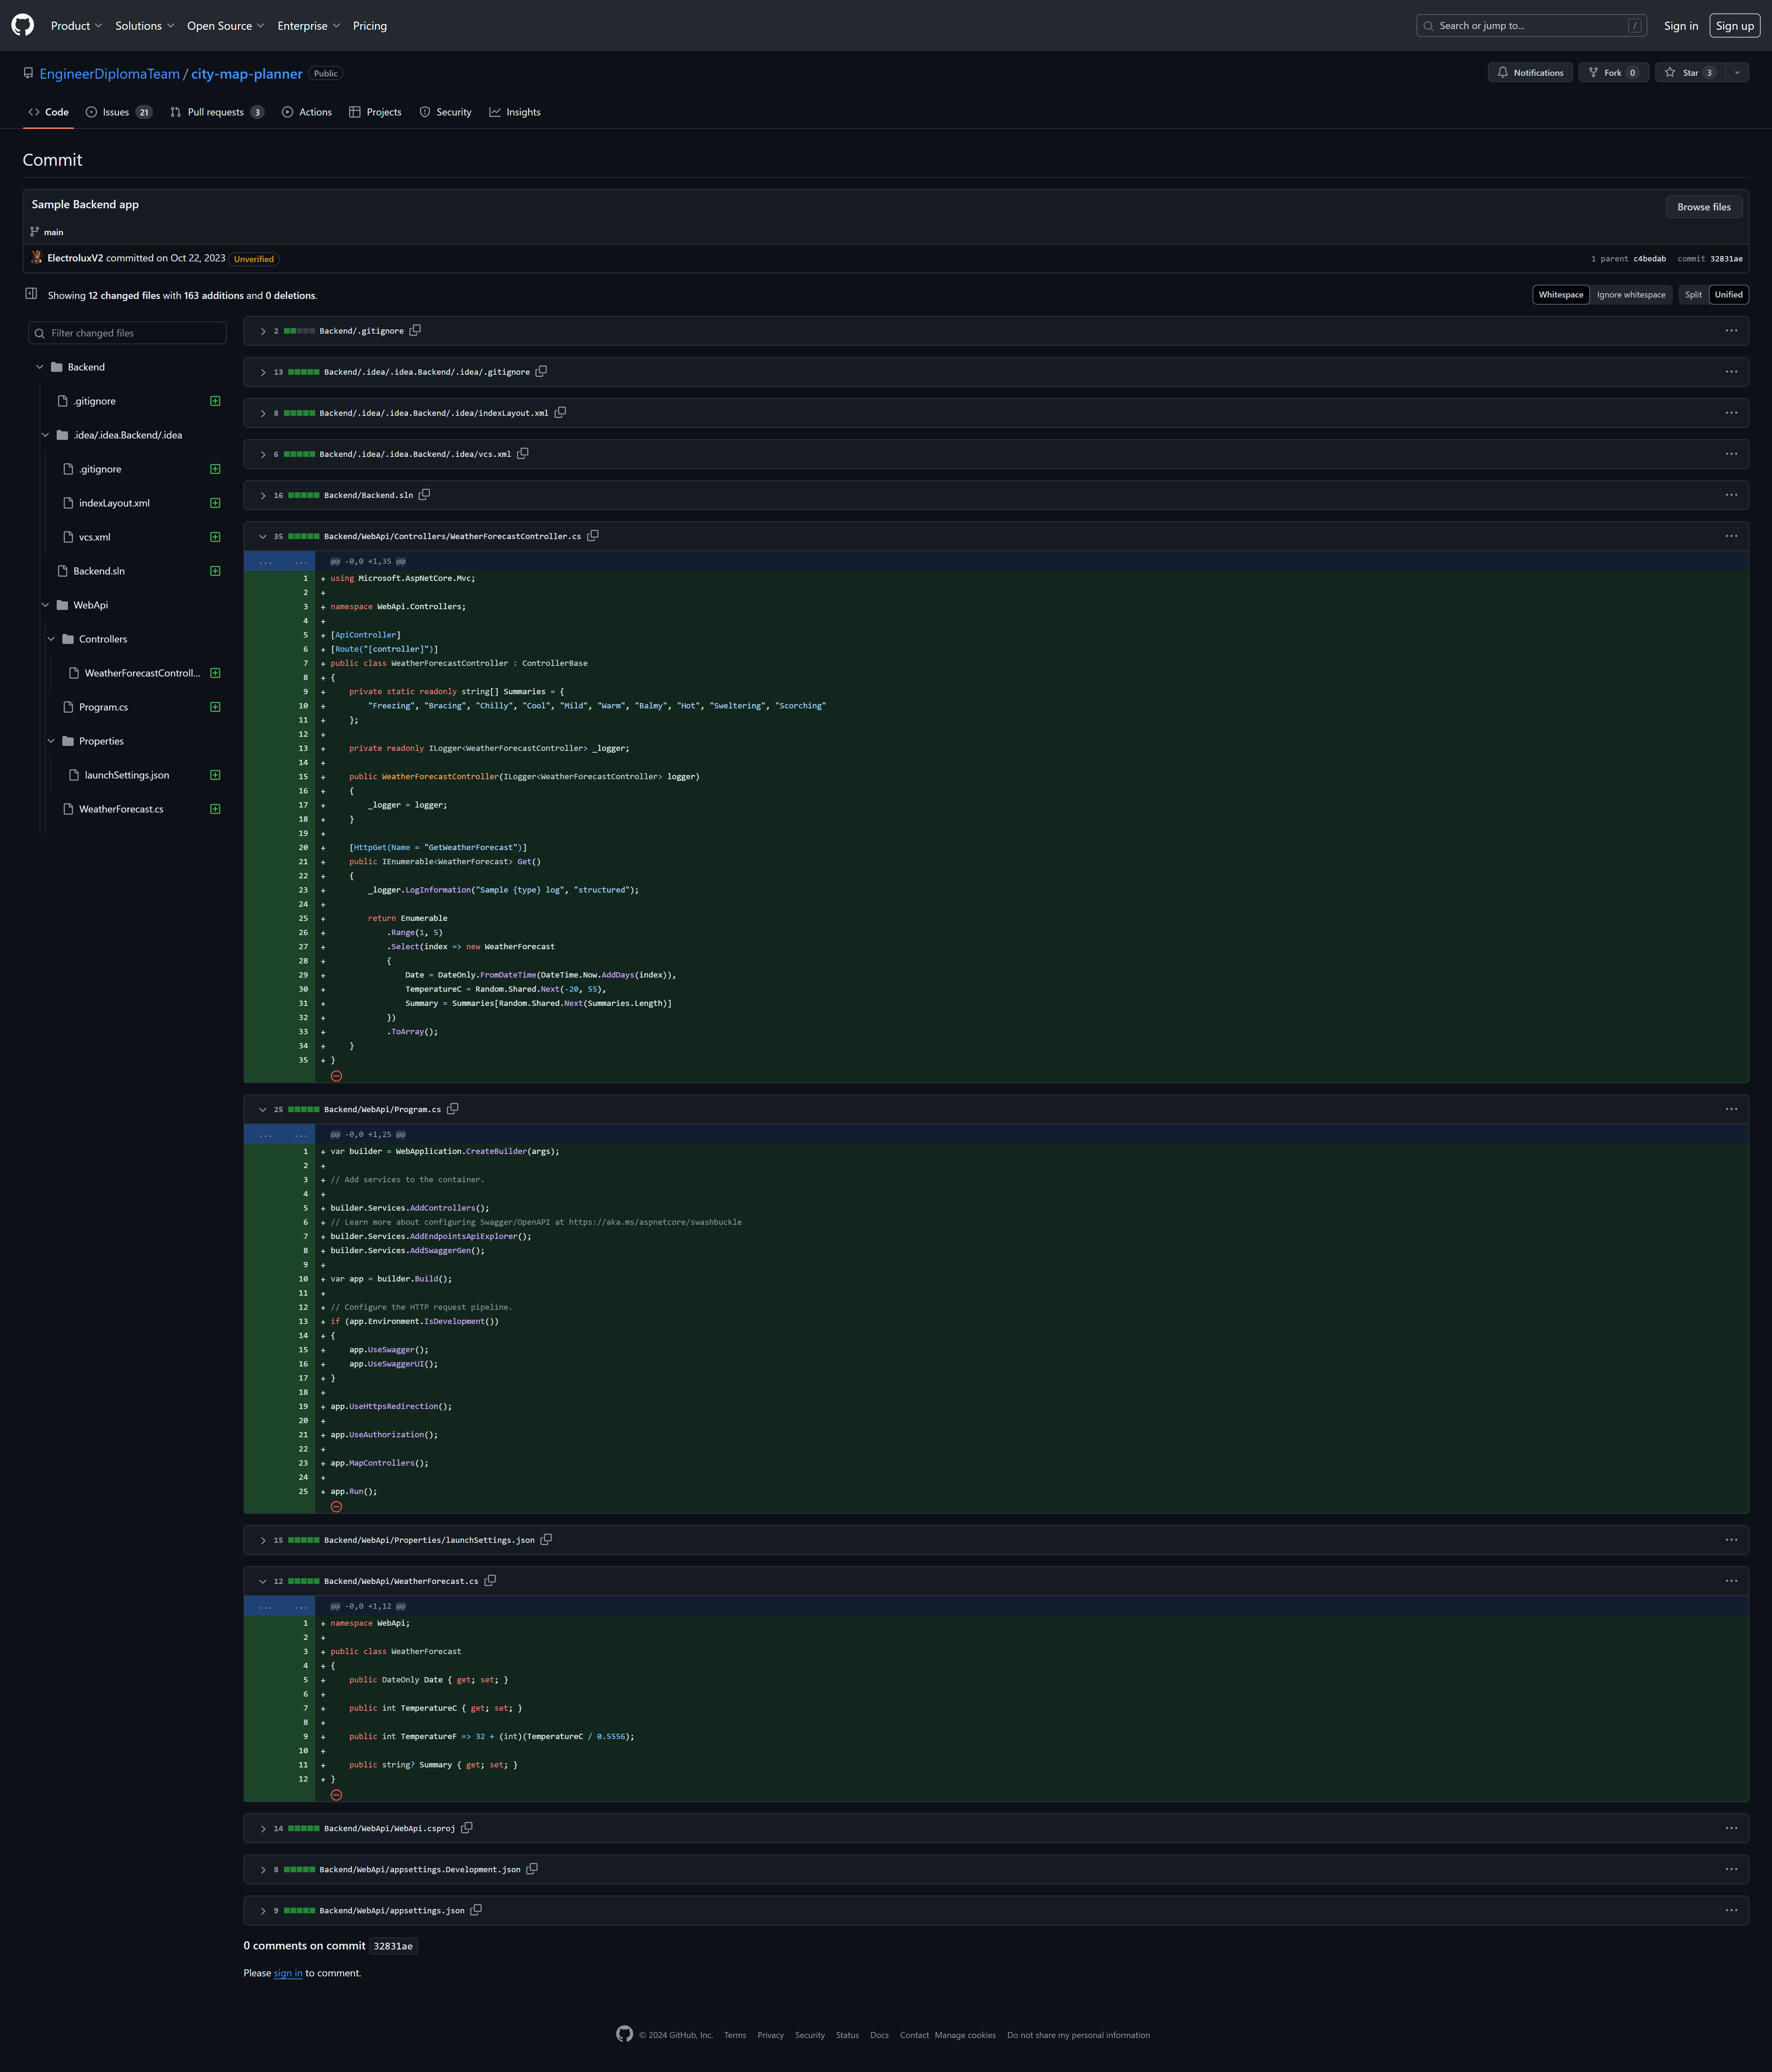
\includegraphics[width=1\textwidth]{attachments/1}
        \caption{Wykonane elementy w ramach pierwszego przyrostu}
        \label{fig:figure1}
        \end{figure}
    \item frontend z ustaleniem wyglady aplikacji o oparcie Material design + api example;
    \begin{figure}[H]
        \centering
        \includegraphics[width=1\textwidth]{attachments/2}
        \caption{Wykonane elementy w ramach pierwszego przyrostu}
        \label{fig:figure2}
        \end{figure}
    \item Potok ciągłego wdrożenia opisane w rozdziale 6.6;
\end{itemize}
 
Opis w czasie wykonanych zadań przestawia wykres Gantt'a
\begin{figure}[H]
    \centering
    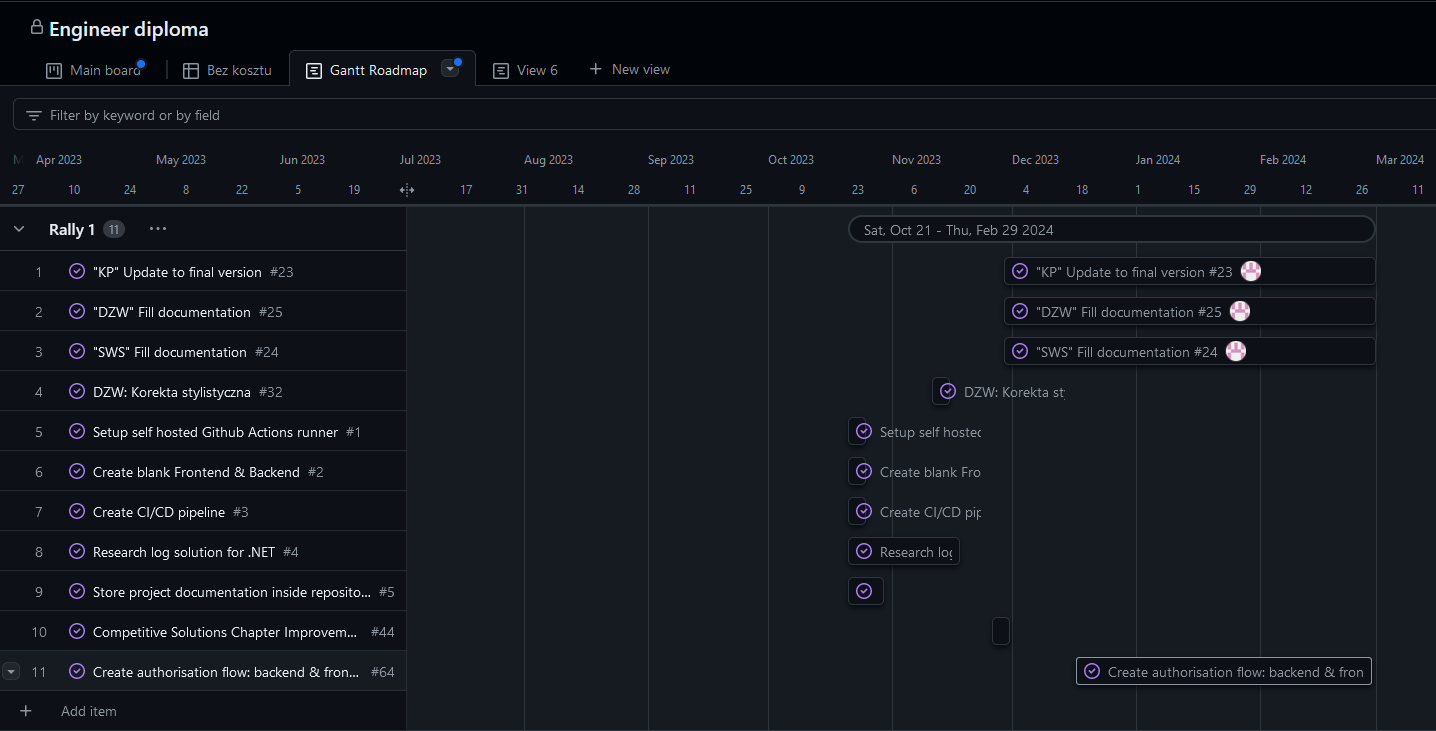
\includegraphics[width=1\textwidth]{attachments/RALLY1}
    \caption{Wykonane elementy w ramach pierwszego przyrostu}
    \label{fig:figure3}
    \end{figure}

    \subsection{Przyrost II - utworzenie widoku mapy, w tym integracja  Overpass}
    \label{sec:przyrost2}

    W ramach tego przyrostu drugiego wykonano elementy, pomiędzy każdym przedstawiono fragmenty wybranych implementacji:
    \begin{itemize}
        \item integracja klienta Overpass API,
        \begin{figure}[H]
            \centering
            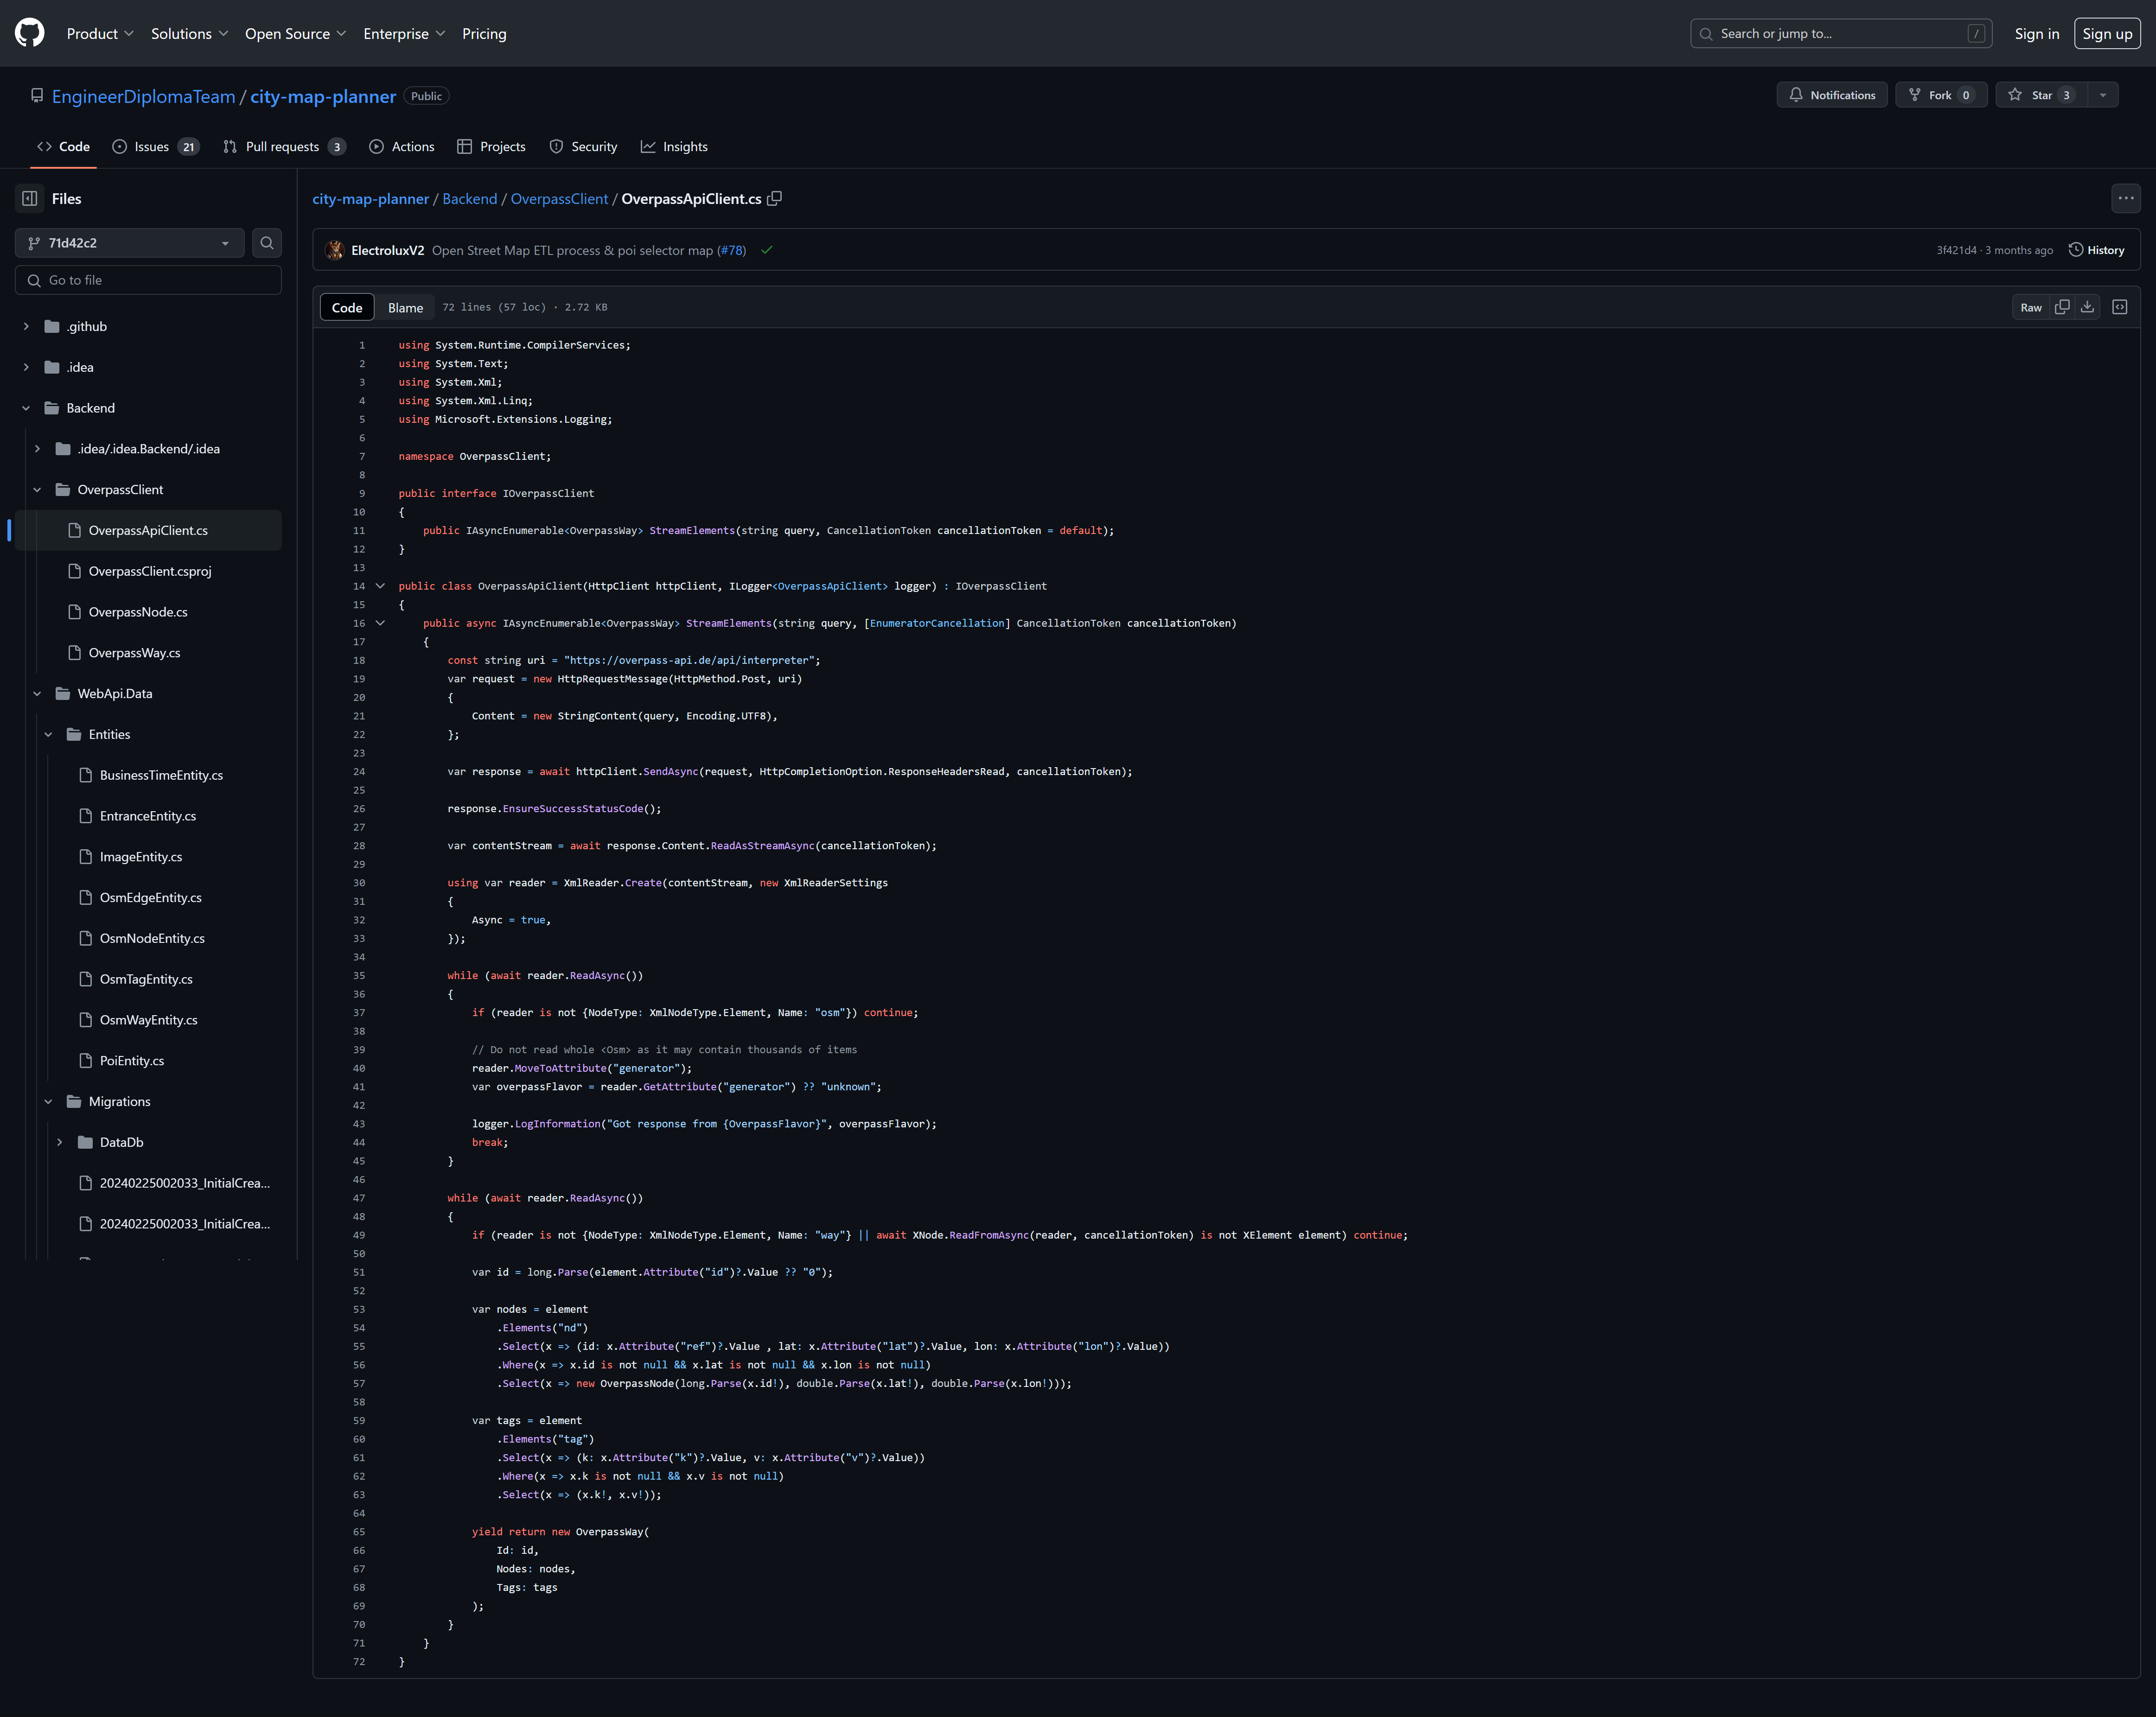
\includegraphics[width=1\textwidth]{attachments/overpassclient}
            \caption{Overpass klient}
            \label{fig:figure4}
            \end{figure}
        \item przygotowanie entities dla Entity Framework Core;
        \begin{figure}[H]
            \centering
            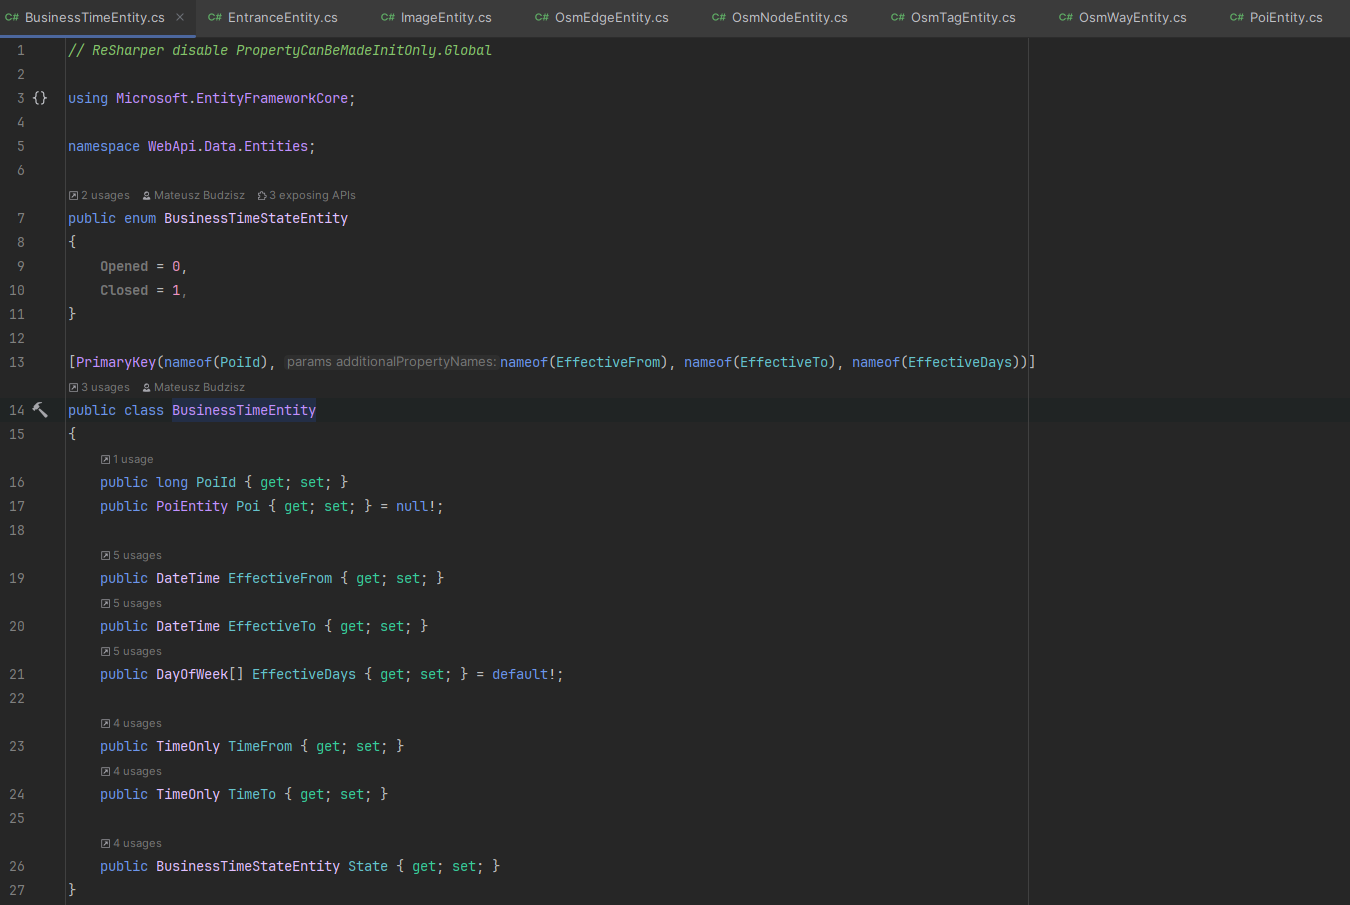
\includegraphics[width=1\textwidth]{attachments/Entity}
            \caption{Fragment klasy BusinessTimeEntity}
            \label{fig:figure5}
            \end{figure}
        \item wykonano kontrolery integrujące usługi
        \begin{figure}[H]
            \centering
            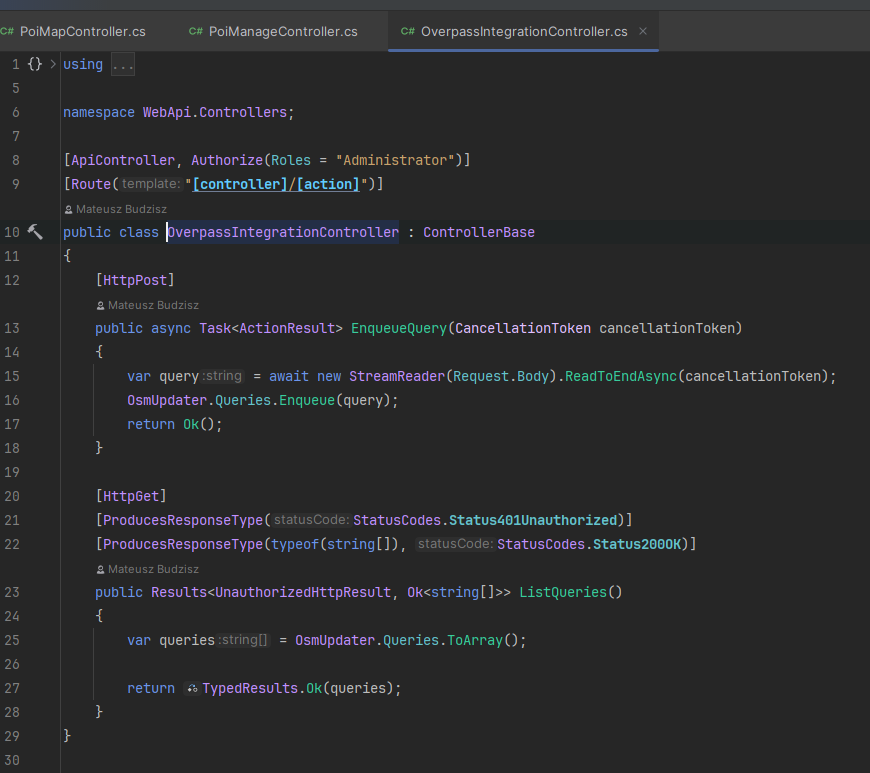
\includegraphics[width=1\textwidth]{attachments/OverpassIntegrationController}
            \caption{Fragment klasy OverpassIntegrationController}
            \label{fig:figure6}
            \end{figure}
        \item implementacja Domain
        \begin{figure}[H]
            \centering
            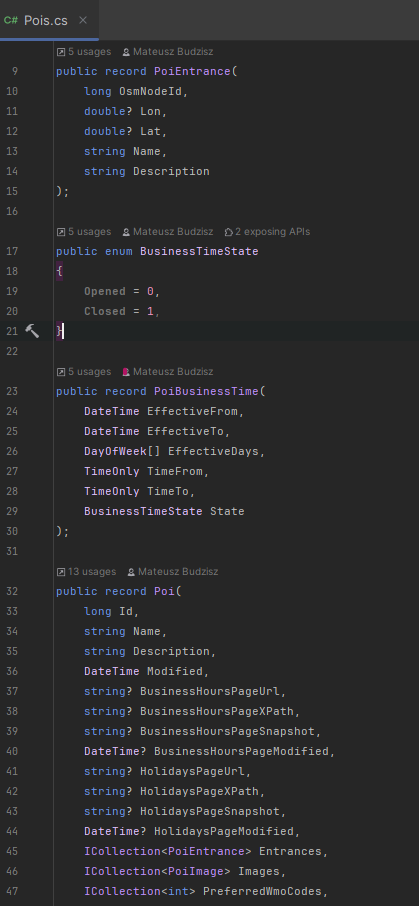
\includegraphics[width=1\textwidth]{attachments/PoisDomain}
            \caption{Fragment klasy Pois}
            \label{fig:figure7}
            \end{figure}
        \item implementacja Dto
        \begin{figure}[H]
            \centering
            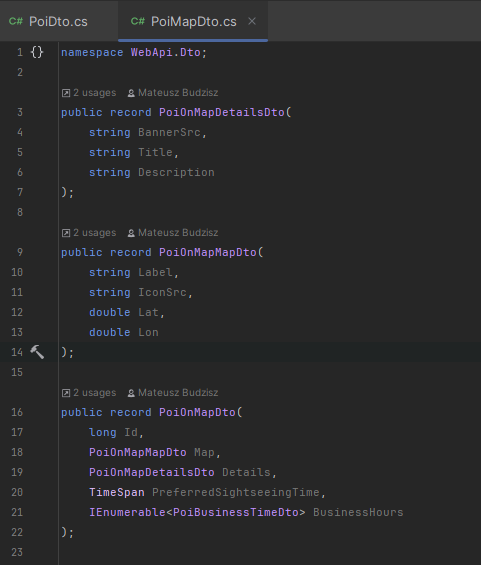
\includegraphics[width=1\textwidth]{attachments/PoiMapDto}
            \caption{Fragment klasy PoiMapDto}
            \label{fig:figure}
            \end{figure}

        \item integracja LeaftModule;
        \begin{figure}[H]
            \centering
            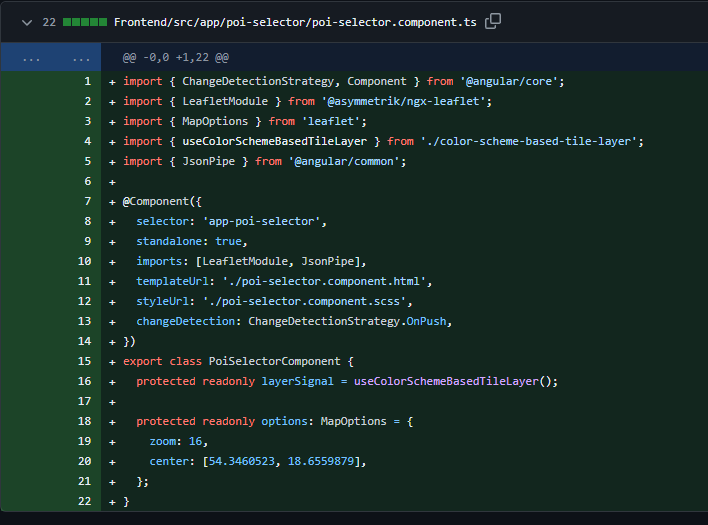
\includegraphics[width=1\textwidth]{attachments/leaflet1}
            \caption{Fragment klasy color-scheme-based-tile-layer}
            \label{fig:figure}
            \end{figure}
            \begin{figure}[H]
                \centering
                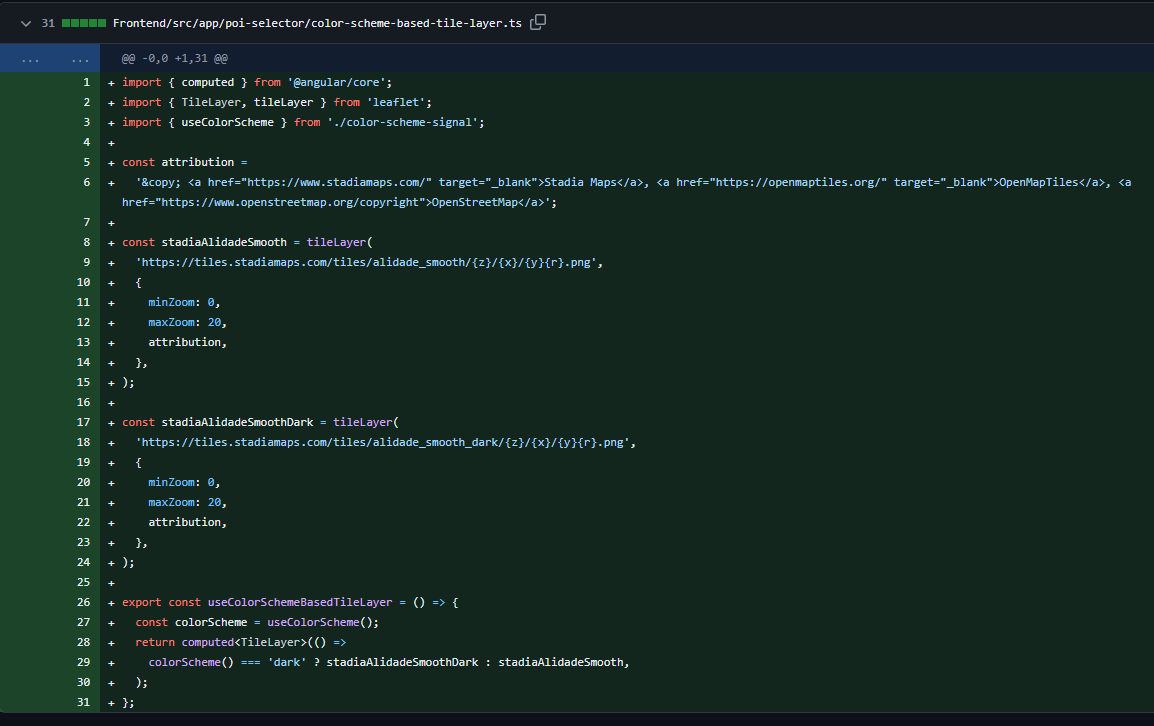
\includegraphics[width=1\textwidth]{attachments/leaflet2}
                \caption{Fragment klasy PoiSelectorComponent}
                \label{fig:figure}
                \end{figure}
    \end{itemize}

    \subsection{Przyrost III - zarządzanie użytkownikiem}
    \label{sec:przyrost3}
    Backend/WebApi/Services/EmailSender.cs
    W ramach tego przyrostu trzeciego wykonano:
    \begin{itemize}
        \item widok logowania;
        \item widok rejestracji z automatycznym potwierdzeniem,
        \begin{figure}[H]
            \centering
            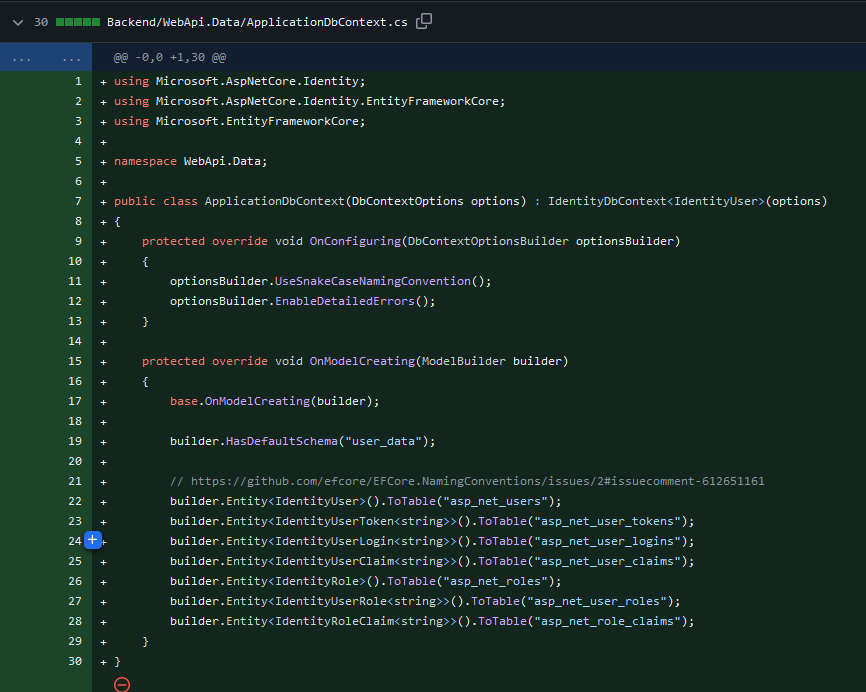
\includegraphics[width=1\textwidth]{attachments/emailsender}
            \caption{Fragment klasy EmailSender z widocznym serwisem potwierdzania rejestracji}
            \label{fig:figure}
            \end{figure}

        \item widok zarządzania kontem;
        \item zaimplementowano autoryzacje logowania po stronie aplikacji oraz bazy danych,
    \begin{figure}[H]
        \centering
        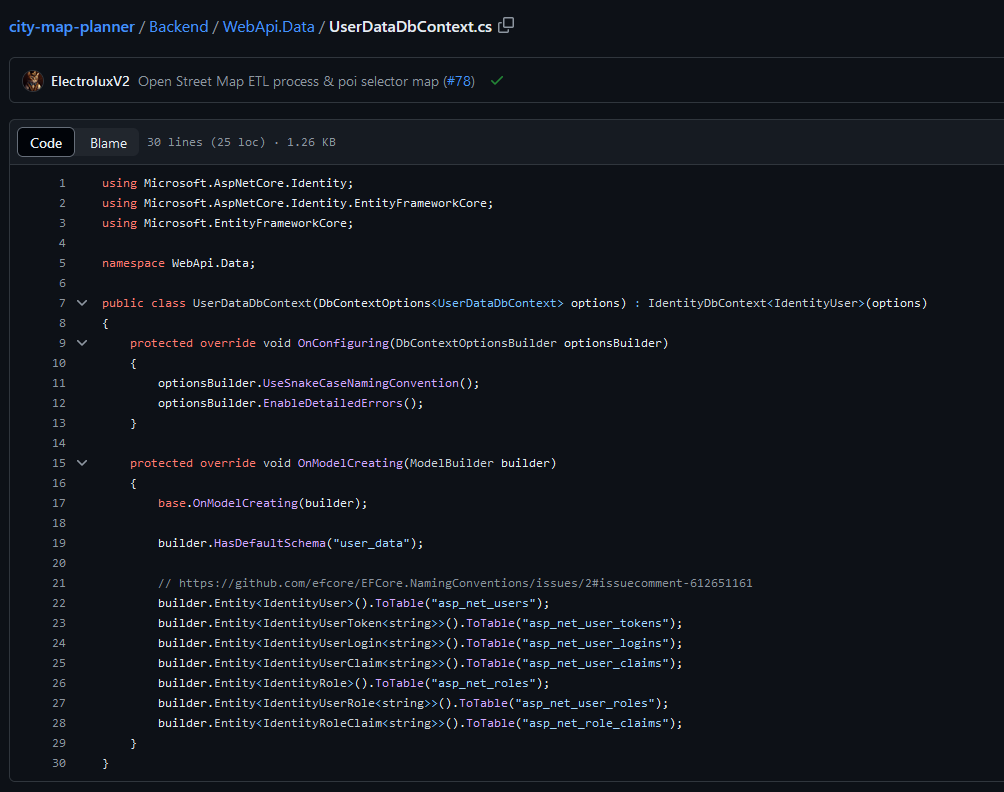
\includegraphics[width=1\textwidth]{attachments/userdb}
        \caption{Fragment klasy UserDataDbContext}
        \label{fig:figure}
        \end{figure}
    \end{itemize}

    %https://github.com/EngineerDiplomaTeam/city-map-planner/tree/b85c21829a74f57ce20414a7fa3ab3a398ad9833/Backend/WebApi/Extensions
    %https://github.com/EngineerDiplomaTeam/city-map-planner/commit/bbdbb4fdca805acd2438365551f4f361532bc34d


    \subsection{Przyrost IV - algorytm Trasy - \glslink{poidef}{POI}}
    \label{sec:przyrost4}

    W ramach tego przyrostu czwartego wykonano:
    \begin{itemize}
        \item dodanie \glslink{poidef}{POI} na mapie uzwgledniając wszystkie podstawowe informacje;
        \item dodanie algorytmu przeszukania trasy pomiędzy \glslink{poidef}{POI};
        \item dodanie ekranu koszyka z \glslink{poidef}{POI};
        %https://github.com/EngineerDiplomaTeam/city-map-planner/commit/88c32b690c76b113173d056ec0be1fa74c81709a#diff-ede64cf229dabd7c007a109c15db77bcacd008a0cf42e1eacca43c3e3da9af97
        \item dodanie indywidualnych zdjeć;
        %https://github.com/EngineerDiplomaTeam/city-map-planner/commit/354caede1081fe73ca98350bd1aceff95c7df8c9
        \item wykonano liste przykładowych atrakcji w Gdańsku
    \end{itemize}


    \subsection{Przyrost V - zarządzanie POI i kalendarz podróży}
    \label{sec:przyrost5}

    W ramach tego przyrostu piątego wykonano:
    \begin{itemize}
        \item integracja chatGPT do inportowania aktualnych o atrakcjach;
        % https://github.com/EngineerDiplomaTeam/city-map-planner/commit/989c85a11ceb0f7f9951f04838e4464c0a47d070
        \item dodanie ekranu kalendarza podróży
        \item Widok podsumowania podróży
        %https://github.com/EngineerDiplomaTeam/city-map-planner/commit/796bac2b6bc5db568a7aabc7dcdef299117c2da2
        \item integracja aplikacji oraz bazy danych z API pogodowym
        %https://github.com/EngineerDiplomaTeam/city-map-planner/commit/1f899291a34701bfa61bfc0b39fd558b628bb966
        \item poprawienie widoku kalendarza
       % https://github.com/EngineerDiplomaTeam/city-map-planner/commit/a3d894bcbf5c319bb2cd109a9b2c3e58db29ef56
    \end{itemize}

    \subsection{Przyrost VI - widok wszystkich atrakcji integracja pogody}
    \label{sec:przyrost5}

    W ramach tego przyrostu szóstego wykonano:
    \begin{itemize}
        \item integracja pogody widoku na przeglądarce internetowej;
        \item widok listy wszystkich POI
    \end{itemize}


	%! Author = Wiktor Rostkowski, Mateusz Budzisz
%! Date = 29/04/2024

\chapter{Testy}
\label{ch:testy}

\section{Testy jednostkowe}
\label{sec:testy-jednostkowe}
W ramach projektu potok frontend wykonał 151 testów. \newline
W ramach projektu potok backend wykonał 159 testów. \newline
W ramach projektu potok dokumentacja wykonał 328 testów. \newline

\section{Testy wydajnościowe}
\label{sec:testy-wydajnosciowe}
Lighthouse
\section{Testy funkcjonalne}
\label{sec:testy-funkcjonalne}

\begin{figure}[H]
    \centering
    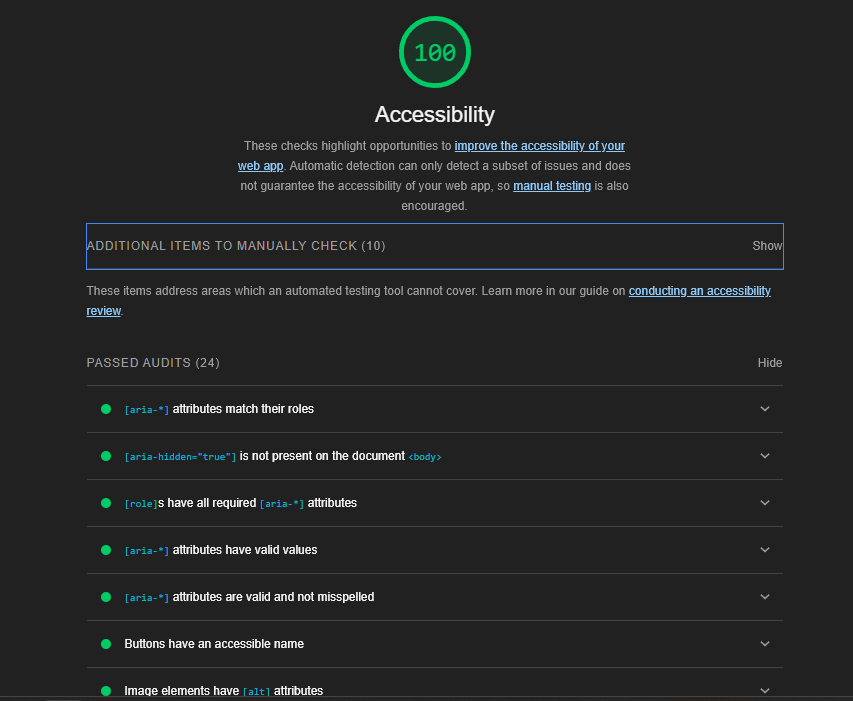
\includegraphics[width=1\textwidth]{attachments/testy-dostepnosci}
    \caption{Widok testu dostępności dla naszej aplikacji}
    \label{fig:testy-dostepnosci}
    \end{figure}
	%! Author = Mateusz Budzisz
%! Date = 26/05/2024

\chapter{Prezentacja systemu}
\label{ch:prezentacja-systemu}



\subsection{Widok głównej stron}
\label{sec:mapawidok}
\begin{figure}[H]
    \centering
    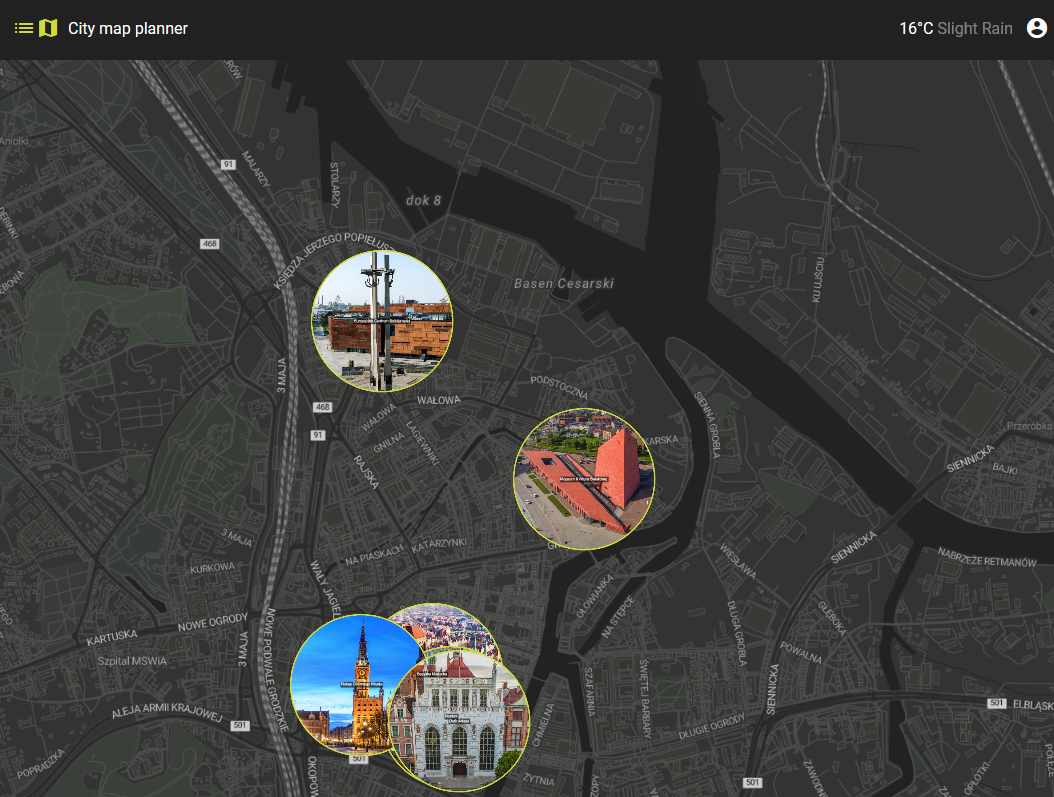
\includegraphics[width=1\textwidth]{attachments/mapawidok}
    \caption{Widok głównej strony}
    \label{fig:mapawidok}
    \end{figure}

\subsection{Widok pojedynczej atrakcji}
\label{sec:atrakcjawidok}
\begin{figure}[H]
        \centering
        \includegraphics[width=1\textwidth]{attachments/atrakcjawidok}
        \caption{Widok pojedynczej atrakcji}
        \label{fig:mapawidok}
\end{figure}

\subsection{Widok koszyka}
\label{sec:koszyk}
    \begin{figure}[H]
        \centering
        \includegraphics[width=1\textwidth]{attachments/koszyk}
        \caption{Widok koszyka}
        \label{fig:koszyk}
\end{figure}

\subsection{Widok kalendarza}
\label{sec:atrakcjawidok}
\begin{figure}[H]
        \centering
        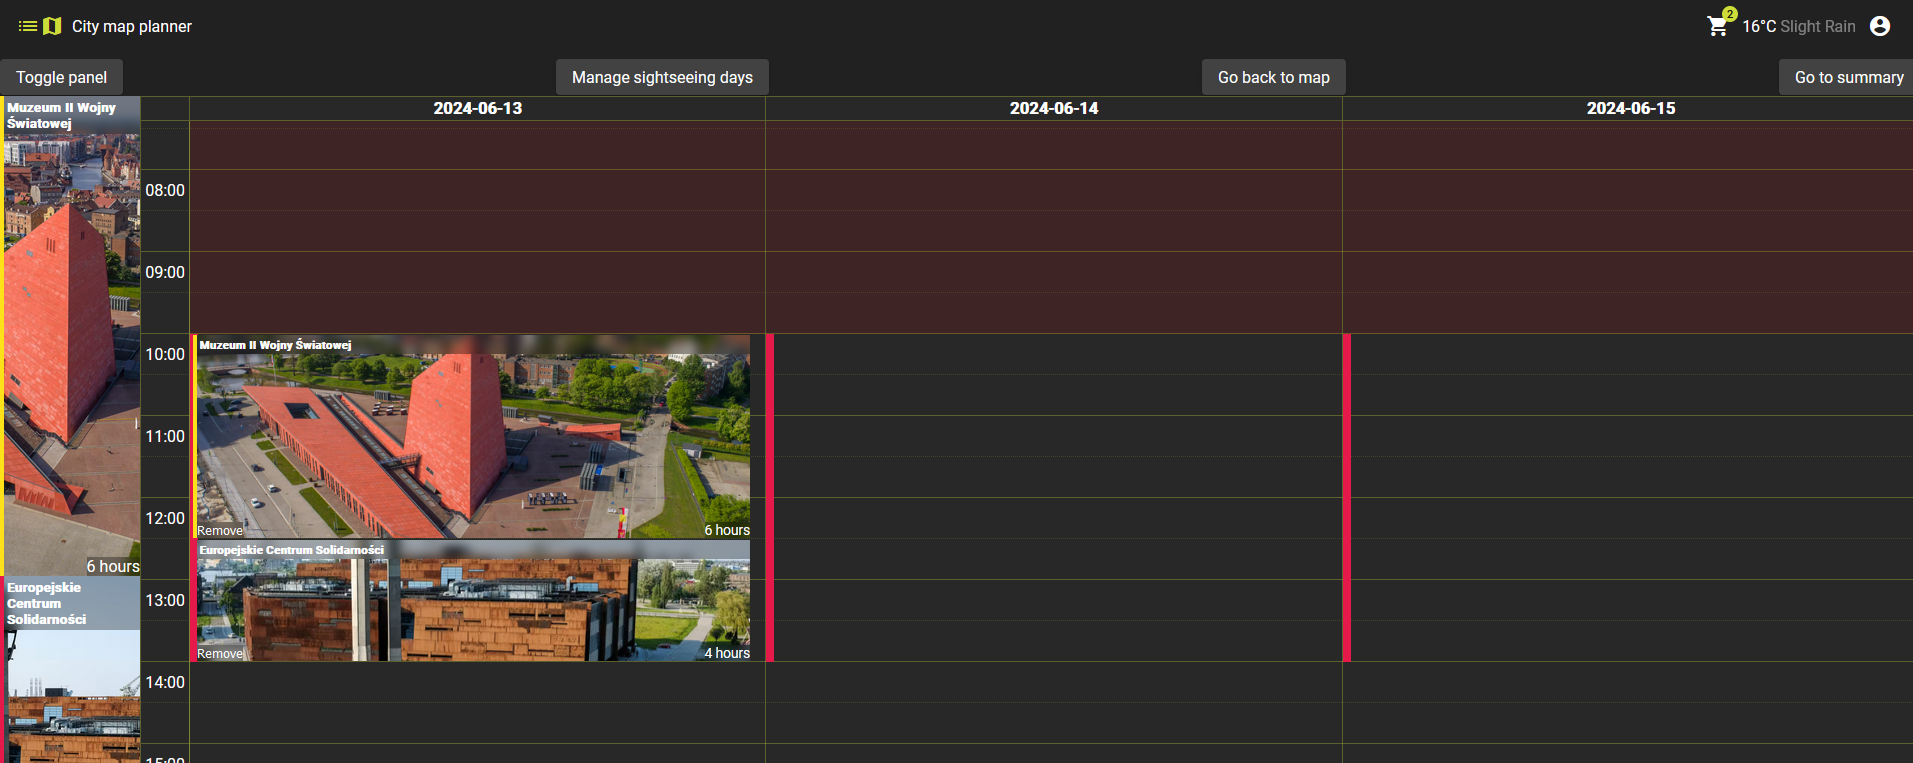
\includegraphics[width=1\textwidth]{attachments/kalendarz}
        \caption{Widok kalendarza}
        \label{fig:kalendarz}
\end{figure}
\subsection{Widok podsumowania}
\label{sec:atrakcjawidok}
\begin{figure}[H]
    \centering
    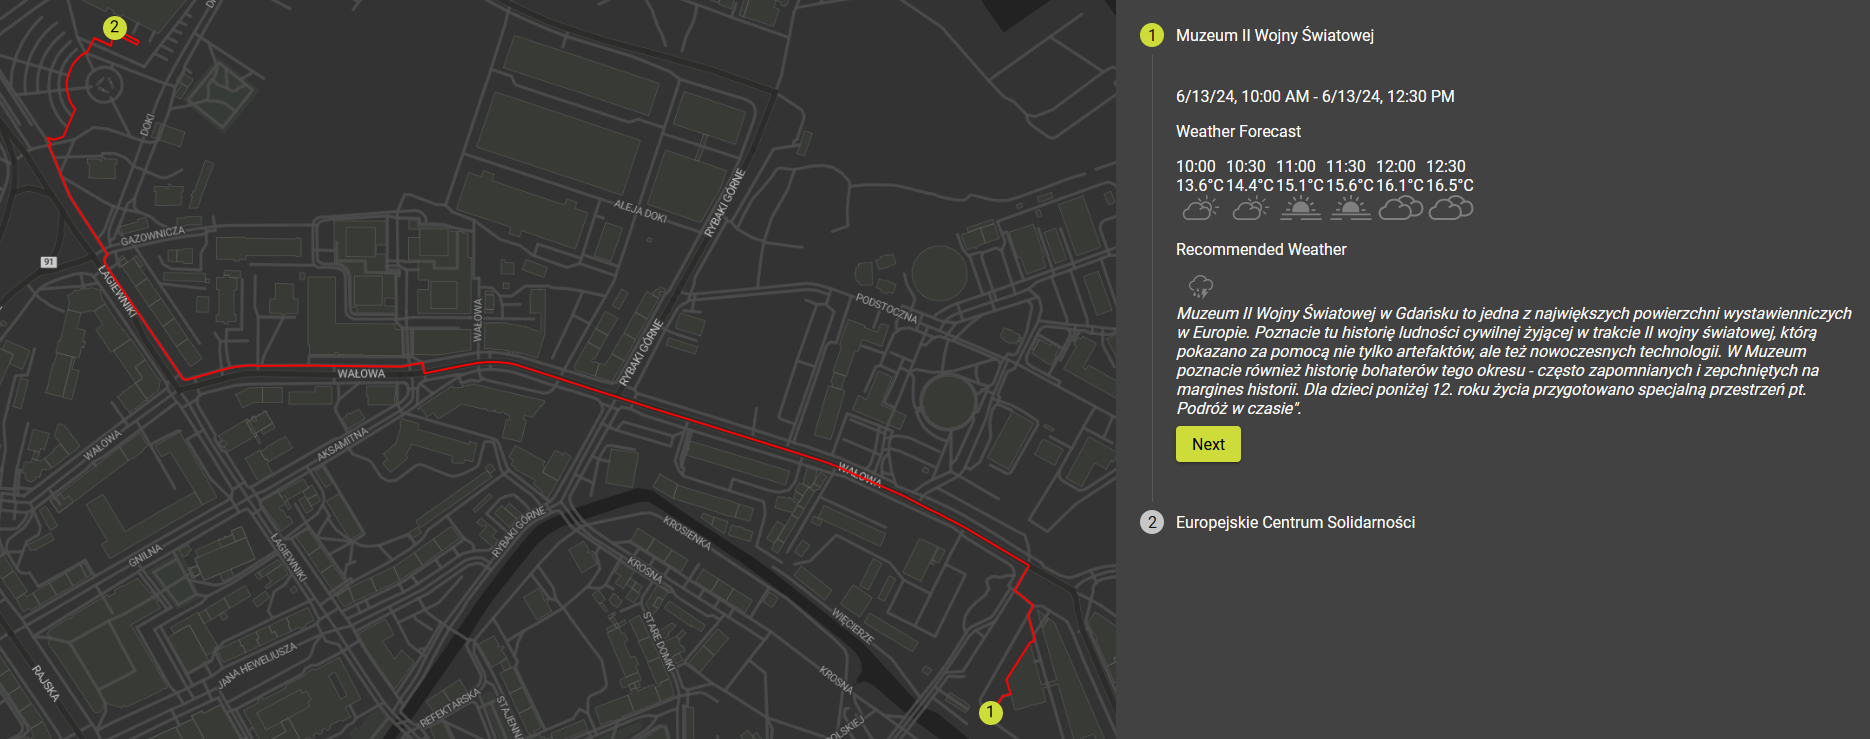
\includegraphics[width=1\textwidth]{attachments/podsumowanie}
    \caption{Widok podsumowanie}
    \label{fig:podsumowanie}
\end{figure}
\subsection{Widok Listy POI}
\label{sec:poilist}

\begin{figure}[H]
    \centering
    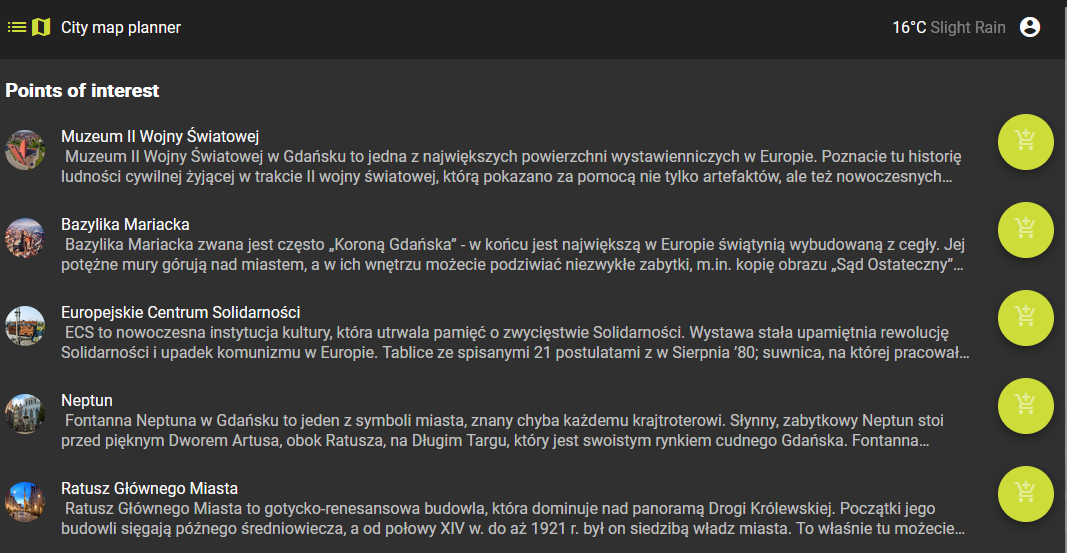
\includegraphics[width=1\textwidth]{attachments/poilist}
    \caption{Widok listy wszystkich dostępnych atrakcji}
    \label{fig:poilist}
\end{figure}


\subsection{Widok Listy POI}
\label{sec:user}

\begin{figure}[H]
    \centering
    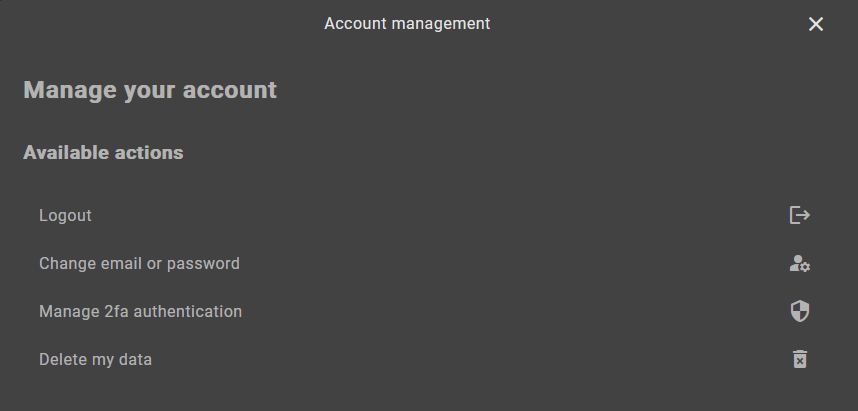
\includegraphics[width=1\textwidth]{attachments/user}
    \caption{Widok panelu zarządzania użytkownikiem}
    \label{fig:user}
\end{figure}

\subsection{Widok Logowania}
\label{sec:logowanie}

\begin{figure}[H]
    \centering
    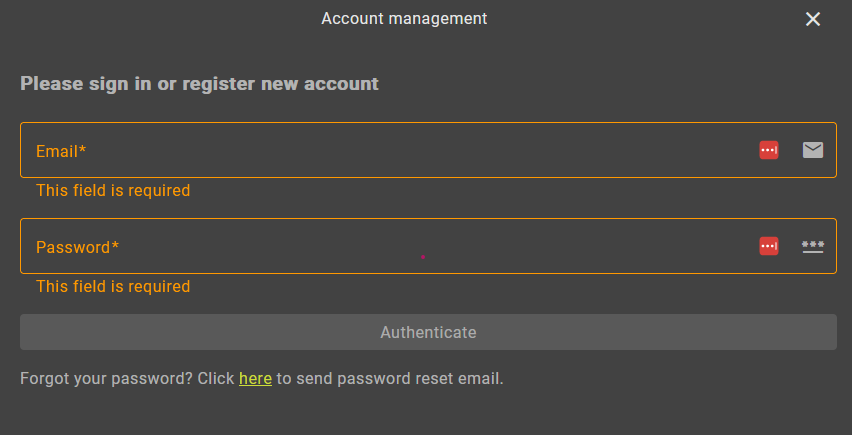
\includegraphics[width=1\textwidth]{attachments/logowanie}
    \caption{Widok panelu logowania}
    \label{fig:logowanie}
\end{figure}

\subsection{Widok zarządzania wszystkimi POI}
\label{sec:manage}

\begin{figure}[H]
    \centering
    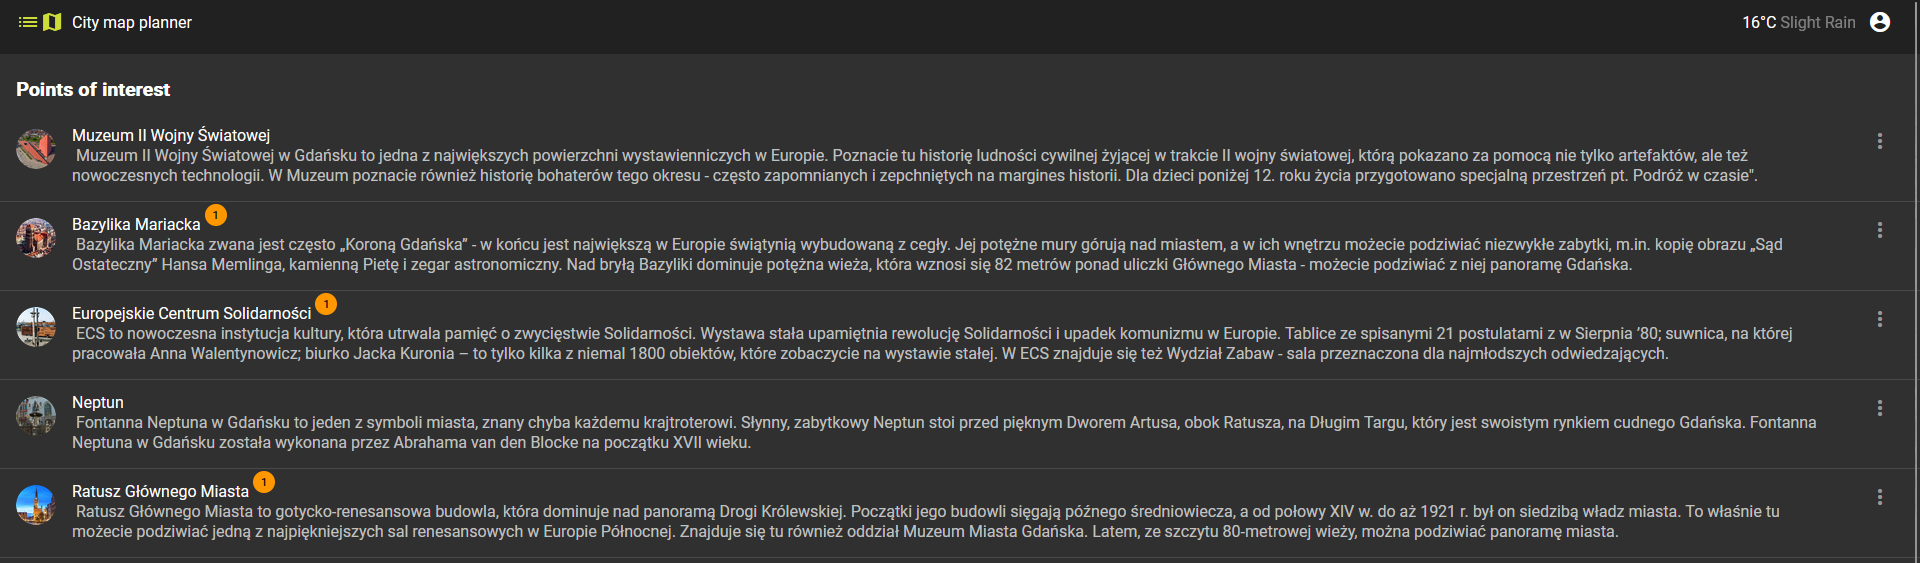
\includegraphics[width=1\textwidth]{attachments/poi-manage}
    \caption{Widok panelu zarządzania wszystkimi POI}
    \label{fig:poi-manage}
\end{figure}

\begin{figure}[H]
    \centering
    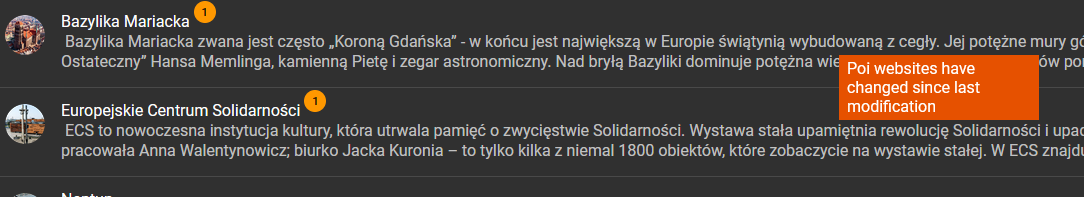
\includegraphics[width=1\textwidth]{attachments/poi-notify}
    \caption{Informacja o potrzebie sprawdzenia aktualności danych}
    \label{fig:ManageNofify}
\end{figure}

\begin{figure}[H]
    \centering
    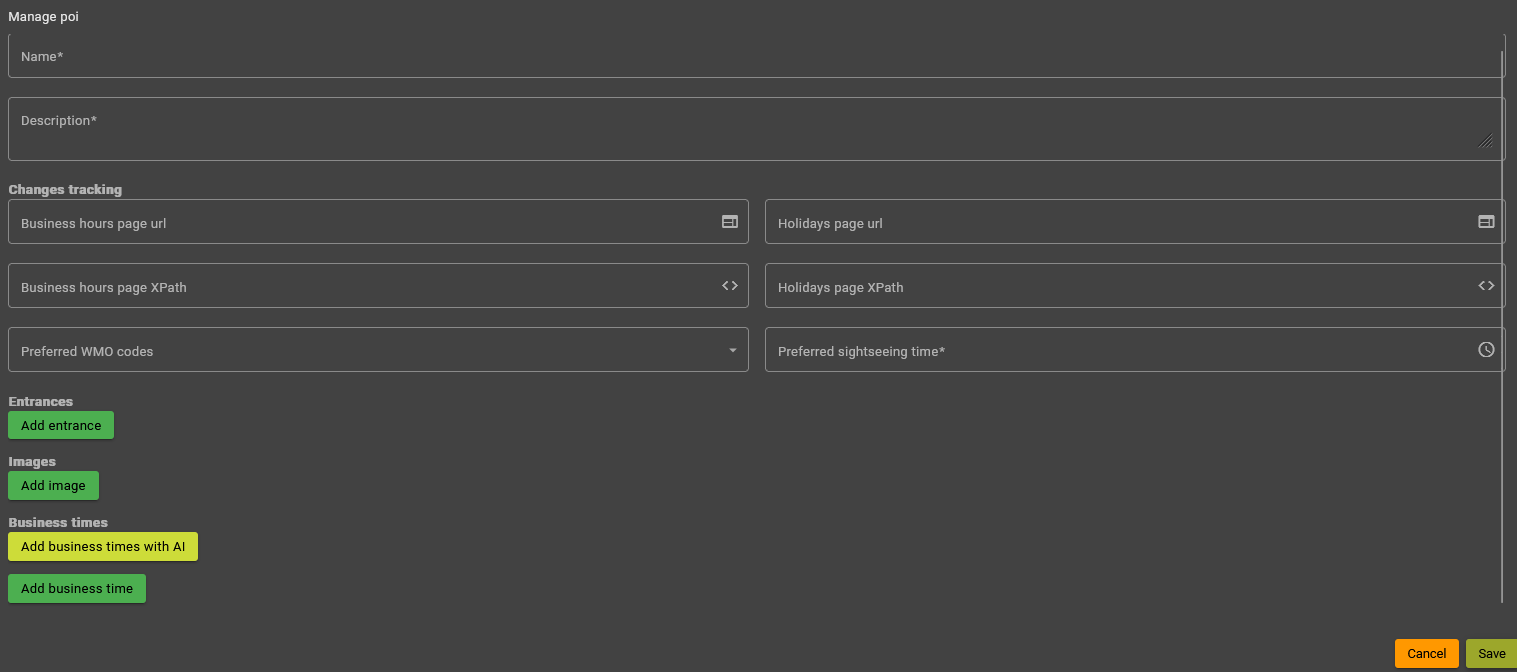
\includegraphics[width=1\textwidth]{attachments/addpoi}
    \caption{Widok panelu dodawania POI}
    \label{fig:ManageNofify}
\end{figure}
	%! Author = Wiktor Rostkowski, Mateusz Budzisz
%! Date = 29/04/2024

\chapter{Podsumowanie}
\label{ch:podsumowanie}

\section{Napotkane wyzwania}
\label{sec:napotkane-wyzwania}

Największym wyzwaniem, z jakim zespół projektowy musiał się zmierzyć, był częściowy rozpad grupy,~w~wyniku którego zespół zmniejszył się o połowę.
To znaczące uszczuplenie liczby członków wpłynęło na zdolność zespołu do realizacji wszystkich zaplanowanych funkcjonalności.\newline
W rezultacie projekt nie był~w~stanie~w~pełni zrealizować integracji z komunikacją miejską~w~Gdańsku, co było jedną z głównych funkcji przewidzianych~w~początkowym planie.
Ograniczenia te zmusiły zespół do priorytetyzacji innych elementów projektu oraz do poszukiwania alternatywnych rozwiązań, aby sprostać ograniczeniom zasobów~i~czasu.

Drugim największym wyzwaniem była implementacja kalendarza, który umożliwia planowanie zwiedzania~w~wybrane dni za pomocą funkcji przeciągnij~i~upuść.
Kalendarz ten uwzględnia godziny otwarcia atrakcji turystycznych oraz proponowany czas zwiedzania każdej atrakcji.
Algorytm kalendarza musi pilnować wszystkich tych ograniczeń, aby zaplanowany harmonogram był możliwy do zrealizowania~w~rzeczywistości.
Dodatkowo funkcjonalność  możliwości zmiany czasu przeznaczonego na zwiedzanie przez użytkownika wprowadziła kolejny poziom skomplikowania, wymagając dynamicznej aktualizacji planu.
Ta funkcjonalność musiała również uwzględniać różne scenariusze~i~wyjątkowe przypadki, takie jak zmiany godzin otwarcia atrakcji~w~dni świąteczne czy nieprzewidziane zamknięcia, co dodatkowo komplikowało implementację.

\begin{figure}[H]
    \centering
    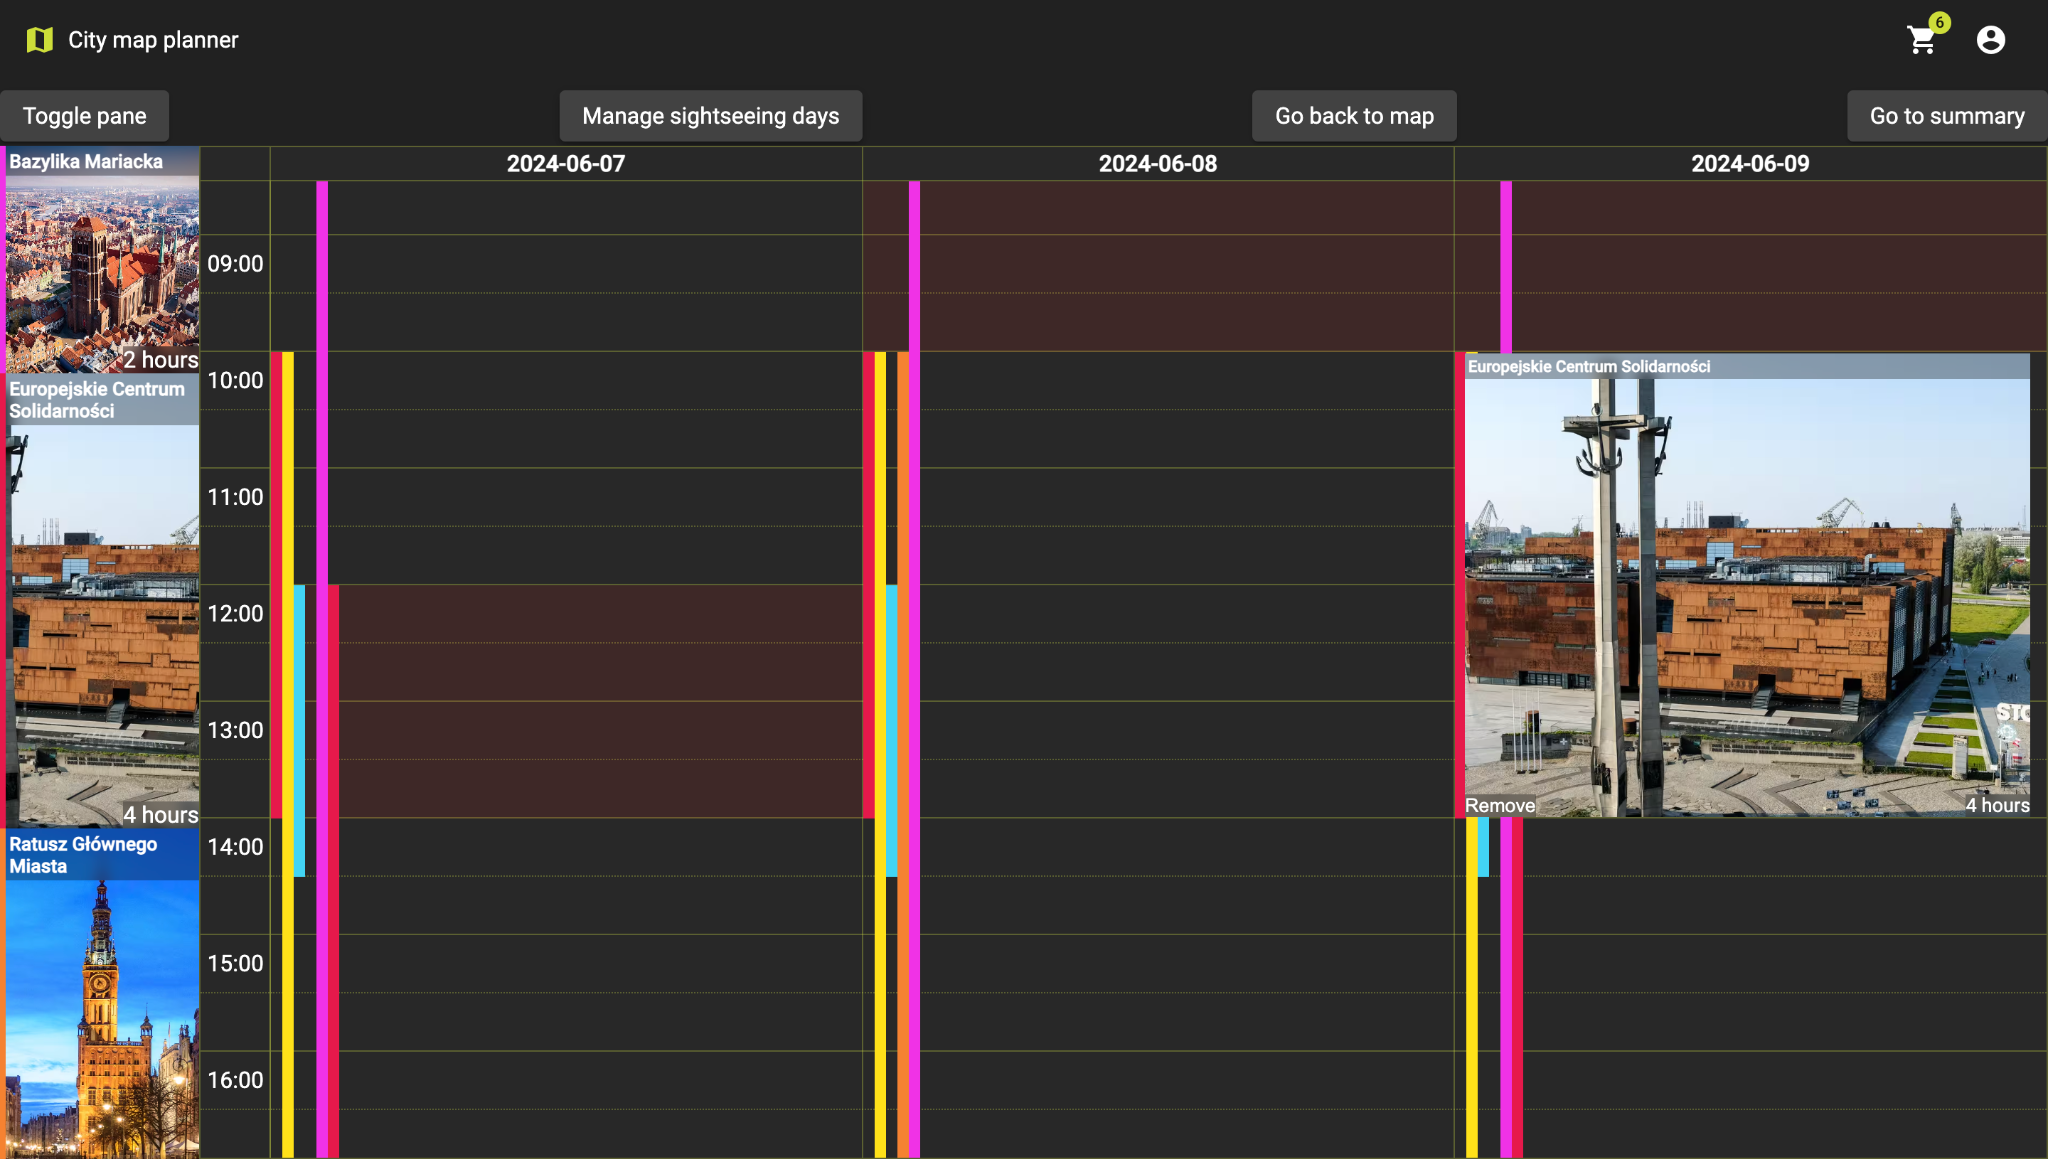
\includegraphics[width=1\textwidth]{attachments/t1}
    \caption{Screenshot przykładowego użycia kalendarza}
\end{figure}

Trzecim wyzwaniem, przed którym stanął zespół projektowy, była integracja menedżera punktów zainteresowania (POI) ze sztuczną inteligencją.
System co godzinę zapisuje snapshot stron internetowych atrakcji~i~porównuje je z wcześniejszymi wersjami~w~celu wykrycia zmian. \newline
W przypadku wykrycia zmian, dane są przesyłane do modelu GPT-4 od OpenAI~w~celu ekstrakcji godzin otwarcia, co częściowo automatyzuje proces aktualizacji informacji.
Sztuczna inteligencja zwraca dane~w~formacie tabelki markdown z wartościami wymagającymi normalizacji.
Przetwarzanie tych zdenormalizowanych danych przed zapisaniem ich do finalnej tabeli~w~bazie danych stanowiło znaczące wyzwanie.
Ponadto konieczne było uwzględnienie~i~pokrycie wielu przypadków anomalii generowanych przez AI, co dodatkowo skomplikowało ten proces.
Wyzwanie to wymagało nie tylko solidnej wiedzy technicznej, ale także elastyczności~w~dostosowywaniu systemu do różnych formatów~i~źródeł danych.

\begin{figure}[H]
    \centering
    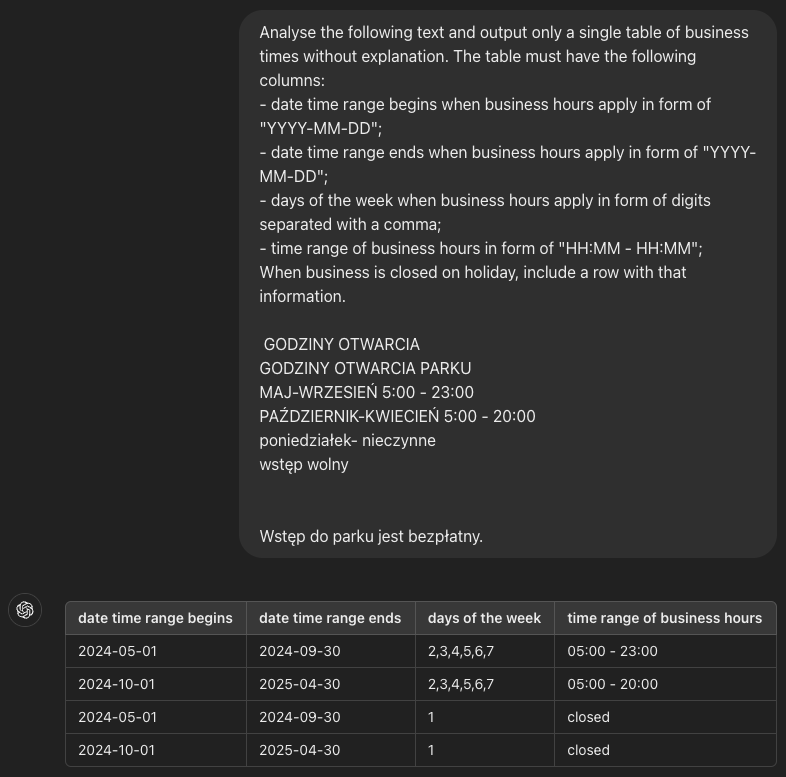
\includegraphics[width=1\textwidth]{attachments/t2}
    \caption{Przykład analizy AI}
\end{figure}

\section{Łączny nakład pracy}
\label{sec:laczny-naklad-pracy}

Łączny czas poświęcony przez aktualny członków zespołu na realizację tego projektu wyniósł 380 godzin.
Ten czas obejmował szeroki zakres działań,~w~tym analizę wymagań, projektowanie architektury systemu, implementację poszczególnych modułów, testowanie funkcjonalności oraz naprawianie błędów.
W ramach tych godzin zespół przeprowadzał także spotkania planistyczne~i~statusowe, konsultacje z interesariuszami, a także sesje programowania ekstremalnego, aby zapewnić, że wszystkie elementy projektu są zgodne z założeniami~i~spełniają oczekiwania użytkowników końcowych.

\section{Indywidualne wkłady pracy}
\label{sec:indywidualne-wklady-pracy}

\subsection{Mateusz Budzisz}
\label{subsec:mateusz-budzisz}

Bezpośrednio na projekt przeznaczyłem 253 godziny.
Jestem autorem pomysłu pracy dyplomowej oraz kierownikiem projektu.
Do moich obowiązków należało: organizacja cotygodniowych spotkań, przygotowanie infrastruktury docelowej, stworzenie~i~utrzymywanie repozytorium oraz ogólnie pojęta organizacja całości projektu.

W znacznej większości zaimplementowałem zarówno backend, jak~i~frontend systemu, co stanowiło kluczowy element techniczny projektu.
Dodatkowo, większość rozdziałów pracy dyplomowej jest mojego autorstwa, co odzwierciedla moje zaangażowanie~i~wkład merytoryczny~w~dokumentację projektu.

Pomimo moich wszelkich starań, aby wspierać innych członków zespołu,~w~tym poprzez propozycje wspólnych sesji programowania oraz udostępnienie prywatnych materiałów szkoleniowych, nie udało mi się przekonać ich do systematycznej pracy na rzecz projektu.
Starałem się aktywnie motywować~i~wspierać zespół, jednak spotkałem się z brakiem odpowiedniego zaangażowania z ich strony.
Moje wysiłki~w~zakresie organizacji~i~koordynacji prac projektowych, jak również znaczny wkład~w~rozwój techniczny~i~dokumentacyjny projektu, były kluczowe dla jego postępu~i~finalizacji.

\subsection{Wiktor Rostkowski}
\label{subsec:wiktor-rostkowski}

W ramach realizowanego projektu byłem odpowiedzialny za fazę przedprojektową oraz kilka kluczowych zadań związanych z jego dalszym przebiegiem.\newline
Moje obowiązki obejmowały opracowanie~i~dokumentację kluczowych etapów projektu,~w~tym rozdziały~w~konspekcie projektu oraz analizę wymagań. \newline
Ponadto, przygotowałem merytoryczne materiały niezbędne do realizacji projektu, zapewniając solidne podstawy teoretyczne~i~praktyczne. \newline
Jednym z moich głównych zadań była integracja pogodowa, którą bezpośrednio przygotowałem zarówno po stronie frontendowej, jak~i~backendowej.\newline
\indent Praca ta wymagała dogłębnego zrozumienia mechanizmów używanych~w~projekcie, co było szczególnym wyzwaniem ze względu na ograniczony czas oraz konieczność nauczenia się niemal wszystkich wykorzystanych technologii od podstaw.
Na bezpośrednie efekty pracy przeznaczyłem 127 godzin. Dodatkowo, aby wykonać te zadania, potrzebowałem poświęcić ponad 60 godzin na przygotowanie merytoryczne~i~zdobycie niezbędnej wiedzy.\newline
Pomimo tych trudności, udało mi się skutecznie zrealizować wszystkie powierzone zadania, przyczyniając się do sukcesu naszego projektu inżynierskiego.

\subsection{Damian i Sebastian Kreft}
\label{subsec:bracia-kreft}
Pomimo licznych prób i wysiłku uczestników, praca nad projektem inżynierskim przyniosła znikome rezultaty. 
Spędzili oni 48 godzin nad elementami, które częściowo zostały uwzględnione w projekcie po~wprowadzeniu poprawek, jednak nie udało 
im się ukończyć wielu istotnych rozwiązań. Mimo podejmowanych kolejnych prób, wymagania projektu okazały się zbyt wymagające. 
W~rezultacie, mimo włożonego wysiłku, efekty ich pracy były minimalne. 
Napotkane trudności podczas realizacji zadań ostatecznie doprowadziły do rezygnacji uczestników z dalszej współpracy


\section{Wnioski}\label{sec:wnioski}
Prace nad projektem rozpoczęły się pod koniec 2023 roku,~w~momencie sformowania zespołu projektowego podczas VI semestru studiów.
Zespół miał na celu ukończenie projektu do 18 czerwca 2024 roku, co wynikało z terminu narzuconego przez uczelnię oraz przyjętego bufora bezpieczeństwa.

Początkowo zespół planował realizację wszystkich zaplanowanych funkcjonalności, opierając się na komercyjnym doświadczeniu większości jego członków.
Niestety, projekt został tylko częściowo zrealizowany zgodnie z założeniami.
Główne trudności pojawiły się~w~momencie, gdy zespół stracił połowę swoich członków, co spowodowało, że zakres projektu stał się zbyt obszerny do ukończenia przez pozostałych członków.

Pomimo tych trudności, projekt zachował spójność graficzną, a jego kod cechuje się wysoką jakością~i~zgodnością ze standardami aplikacji biznesowych.
Zespół zdołał zrealizować minimalny wartościowy produkt, który przejawia duży potencjał na dalszy rozwój, szczególnie jeśli Urząd Miasta Gdańsk byłby zainteresowany jego wdrożeniem.

Wybrana technologia do realizacji projektu nie sprawiała problemów, co pozwoliło na~sprawne przeprowadzenie prac.
Metodologia RAD (Rapid Application Development) okazała się doskonale dopasowana do charakteru projektu, a wyrafinowane potoki ciągłej integracji aplikacji znacząco przyczyniły się do ukończenia projektu~w~terminie oraz równoległego rozdzielania pracy pomiędzy członków zespołu.

W trakcie realizacji projektu, zespół projektowy zdobył wiele cennych doświadczeń~i~umiejętności, które z pewnością będą miały pozytywny wpływ na ich przyszłe kariery zawodowe.

\chapter*{Załączniki}
\begin{itemize}
    \item Tekst pracy dyplomowej (na płycie CD)
    \item Kod źródłowy projektu (na płycie CD)
\end{itemize}


	\printbibliography[heading=bibnumbered]

\end{document}
